% TÜ Arvutiteaduse instituudi lõputöö eeskuju ver.2.0
% Tõnu Tamme, 2011
% Jüri Kiho, 2003
% todo: joonised, leheküljemõõdud, numbripunktid, mac, lyx
% iconv -f ISO_8859-15 -t UTF-8 -o eeskuju_utf8.tex eeskuju.tex
  %preambula ---------------------------------------------------
  \documentclass [12pt,a4paper]{report}
  \newif\ifutf
  \utftrue %lülitab UTF-8 sisse/välja (\utftrue|\utffalse)
  \usepackage[T1]{fontenc} %täpitäht ühe sümbolina
  \ifutf
  \usepackage[utf8]{inputenc} %sisendfaili koodilehekylg UTF-8
  \usepackage{ut_thesis_utf8}% ver.0.6
  \else
  \usepackage[latin1]{inputenc} %sisendfaili koodilehekylg ISO 8859-1
  \usepackage{ut_thesis}% ver.0.6  
  \fi
  \usepackage[english]{babel}
  %\usepackage{times} %Times New Roman
  \usepackage{indentfirst} %esimene lõik taandega
  \usepackage{graphicx} %joonised failidena
  \usepackage{algorithm2e}
  \usepackage{multirow}
%  \usepackage{pdfcomment}
  \newcommand{\pdfcomment}[1]{}
  \newcommand{\comment}[1]{}
%\usepackage[margin=1in]{geometry}
%\usepackage[showframe]{geometry}
  %\usepackage{url} %\url
  \usepackage{hyperref} %\url+lingid
  \renewcommand\url{\begingroup\urlstyle{rm}\Url} 
  \usepackage{amssymb,amsmath,amsthm}
  \renewcommand{\leq}{\leqslant} %väiksem-või-võrdne märk eriti ilusasti
  \renewcommand{\geq}{\geqslant} %suurem-või-võrdne märk eriti ilusasti
\newcommand{\TM}{$^{\mathrm{tm}}$ }
  \sloppy
  % ------------------------------------------------------------

%\documentclass{report}
%\usepackage{hyperref}
\usepackage{cite}
\usepackage{subcaption}
%\author{Karl Potisepp, Pelle Jakovits, Satish Narayana Srirama}
%\date{\today}
%\title{Large-scale image processing using MapReduce}

\begin{document}

\begin{tiitelleht}
\pealkiri{Large-scale image processing using MapReduce}
\paber{M.Sc. Thesis (30 ECTS)}
\autor{Karl Potisepp}

\teaduskond{Faculty of Mathematics and Computer Science}
\instituut{Institute of Computer Science}
\eriala{Computer Science}

\juhendaja{Pelle Jakovits M.Sc., Satish Narayana Srirama Ph.D.}

\end{tiitelleht}

%\maketitle

\tableofcontents

\chapter{Introduction}

Along with the development of information technology, a constant stream of new applications for solving humanity's problems has also appeared. As we possess more computing power, we can tackle more and more resource-intensive problems such as DNA sequencing, seismic imaging and weather simulations. When looking at these subjects, a common theme emerges: all of these involve either analysis or generation of large amounts of data. While personal computers have gone through a staggering increase in power during the last 20 years, and the processing power even within everyday accessories - such as smartphones - is very capable of solving problems that were unfeasible for supercomputers only a couple of decades ago, analysing the amount of data generated by newest generation scientific equipment is still out of reach in some areas. Moreover, as processor architectures are reaching their physical limitations with regard to how small individual logic gates and components can get, using distributed computing technologies has become a popular way to solve problems which do not fit the confines of a single computer. Supercomputers, GRID-based systems and computing clouds are an example of this approach. Since the fields of distributed computing and image processing are too broad to fully cover in this thesis, this work will focus on the latter of the three with regard to image processing.

Due to the increasing popularity of personal computers, smart televisions, smartphones, tablets and other devices carrying a full-fledged operating system such as Android, iOS or Windows 8, and due to the capability of these devices to act as producers of many kinds of content instead of being passive receivers (like radio and television, for example), there is a need to be able to process that content. Photos need to be resized, cropped and cleaned up, and recorded sound and video need to be shaped into a coherent whole with the aid of editing software. These procedures however may not be something that is best tackled on the same device that was used for recording, because of limiting factors in processing power, storage space and - in some cases - battery life. However with the widespread availability of wireless internet or high-throughput cell phone networks, any of the aforementioned devices can simply upload their data to a more capable computer in order to do necessary processing. 

In many cases the recorded media will be consumed using a different device (for example, viewing holiday photos taken with your smartphone on your computer or smart TV). Therefore, it can be argued that both the steps of transferring media from the recording device and processing it are inevitable anyway. Facebook and YouTube both provide a good example of this scenario: the user can upload their media in more or less in an unprocessed format and the frameworks take care of resizing and re-encoding the media so that it can be consumed by users. However, since these services are very popular, as a consequence the amounts of data that is needed to process are also huge. For example, 72 hours of video data is uploaded to YouTube every minute \cite{youtube_stats}. Even without going into details of video compression or the processing pipelines involved, it is easy to see how even a day's worth of uploads (103 680 hours) quickly becomes unfeasible to compute without resorting to distributed computing.

For solving processing tasks involving data of this scale, engineers at Google (the parent company of YouTube) designed the MapReduce model of distributed computing, of which Apache Hadoop is the most popular open source implementation. It is well known that using the MapReduce model is a good solution for many problems, however judging from the work done in the field of distributed computing with regard to image processing, the suitability of the model for this application not very well known. In this thesis I will describe the MapReduce model, it's implementation in the form of Hadoop, and explore the feasibility of using this technology for doing large scale image processing.

The rest of this work is structured as follows. In the next sections I will describe in more detail the terminology and the problem at hand, chapter 2 will give a brief overview of previous work in this area, describe the MapReduce model and Hadoop. Chapter 3 will focus on describing the two practical use cases, and finally chapters 4 and 5 present an overview of the results and propose future research directions. (TODO obviously rewrite this part after the structure finalised.) %TODO

\section{Problem statement}

Before going deeper into details, I will first specify the size of data I consider to be large-scale with with regard to this work. This requires some grossly simplified description of the architecture of shared amongst all modern computers. It is common knowledge that a computer consists of a processor, memory and a hard drive. The processor performs calculations on the data stored in memory, which has previously been read from a hard drive. It is important to note here that since very many computers are also connected to the Internet, the hard drive in question may reside in a different physical location than the processing unit and memory. Now, it is also known that the data transfer speed between the processor and memory is generally orders of magnitude faster than between memory and hard drive. Similarly, reading from a local hard drive is faster than accessing data from storage in a different computer, due to overhead added by having to communicate over a network.

Therefore, as the size of the data to be processed by one algorithm increases so that the computer no longer can hold all the information in memory, there is a significant decrease in processing speed. Similarly, if the data does not fit on the local hard drive, the processing speed drops due to having to wait for it to be sent in from another computer. While this can be alleviated somewhat by using buffering techniques, the general rule remains the same: it's best if the problem fits within memory, worse if it fits on the local hard drive and worst if the data has to be read across the network. Processing a large image is an example of such a problem.

In this case we are dealing with a microscope image with a resolution of 86273 by 81025 pixels (roughly 6.99 gigapixels), where each pixel is made up of 3 values - red, green and blue. Assuming that each of these values is stored as a 32-bit precision floating point number, the total memory consumption of storing this data in an uncompressed way can easily be calculated:

\begin{center}
$ 86273 * 81025 * 3 * 32$ bits $ = 78.12 $ gigabytes.
\end{center}

At the time of writing this document, most commodity computers do not have the required memory to even store this amount of data, and certainly not to perform any sort of processing with an overhead dependent on the input size, and even though there do exist specialised computers with enough memory for solving this issue, they are significantly more expensive to acquire and maintain. However, our aim is to find out whether it is possible  to process this kind of images using commodity computers in such a way that all the necessary data is stored within memory.

The second case involves a data set of 48469 images totalling 308 GiB (the average image here is a JPEG2000 file around 6.5MiB in size). While the size of the data set is small enough to fit on regular hard drives, and processing the images individually is not a problem, because the average size remains around 13 megapixels, thus requiring roughly only 40 MiB of memory, which is orders of magnitude less than was the case with the large image. In this case, the issue is not so much being able to fit the problem within memory, but rather about being able to process the data quickly enough. Here we depend on the processor - it does not matter how many more images you can fit inside the memory since generally the processor can only work on one image at a time. In reality, this depends on how many cores the processor has and how well the algorithm can take advantage of that, but even with many cores, going through all of the data can be very time-consuming. Therefore, the problem to solve in this case is how to process this data set in an efficient way.

In this section I have established that processing the aforementioned classes of large images or large data sets of regular images can not be done on a single personal computer, because in the first case, they do not fit into memory, and in the second case one computer can not process them fast enough. Neither of these issues can be expected to be solved by advances in computing power, because CPUs are already reaching their theoretical physical limitations  and the scale of data is increasing faster than the processing capabilities of single commodity computers. 

A solution for these problems is turning towards distributed computing, where limitations of a single computer are overcome by combining the resources of many computers to perform one large task. While this approach is not new - supercomputers and computing clusters have existed for many years already - it is only recently that techniques of using commodity computers for distributed processing have gained popularity. In the following I will explain more thoroughly how these technologies could be used to solve image processing tasks.

\subsection{Distributed image processing}

Since this thesis is focused on using the MapReduce model for performing image processing, I will now describe some of the issues that stem from the limitations of this model with regard to images. I will also restrict the problem space to 2-dimensional colour images. This may not seem like much of a change at first, as it is probably the most common definition for an image, yet it allows us to disregard issues related to videos, 3-dimensional meshes and other types of image data that is also studied in the field of image processing. Finally, I will further divide image processing problems into four classes: iterative local and non-local algorithms and non-iterative local and non-local algorithms.

Generally speaking, the MapReduce parallel computing model follows what can be called a divide-and-conquer strategy of parallelised computing. That is, instead of joining together physical resources like processing power, memory and hard drive storage in order to allow the processing software to see these combined devices as one monolithic entity, the problem is divided into independent parts which are then processed separately - usually in different physical or virtual computers - and later joined together to form the output. In the following I will explain how this affects the parallelisation of image processing algorithms.

Local, with regard to image processing, denotes that the computation is performed as a series of small calculations on fixed subsets of the image: typically this means that the value of a pixel in focus is re-calculated using the values of it's neighbouring pixels. It is easy to see how problems like this can be parallelised by virtue of splitting the image into parts, performing the processing, and later putting it back together. Gaussian blurring, which I will briefly describe during the course of this work, is an example of a local processing algorithm. Contrary to local, non-local problems involve larger parts of the image. A good example of non-local processing is object recognition. For example, in order for a trained character recognition algorithm to be able to recognise the letter "A" from an image, it's search window needs to be big enough to encompass the whole letter (see figure \ref{fig_local_nonlocal}). The solution of splitting the image into parts to allow for parallel processing now requires special attention in order to avoid splitting objects into unrecognisable fragments, and in the worst case could be entirely inapplicable if the object to be classified takes up the whole image.

\begin{figure}[h]
\begin{center}
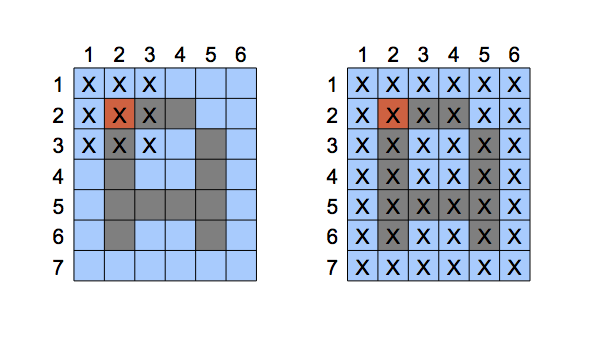
\includegraphics[]{local_nonlocal.eps} %TODO render with PDF
%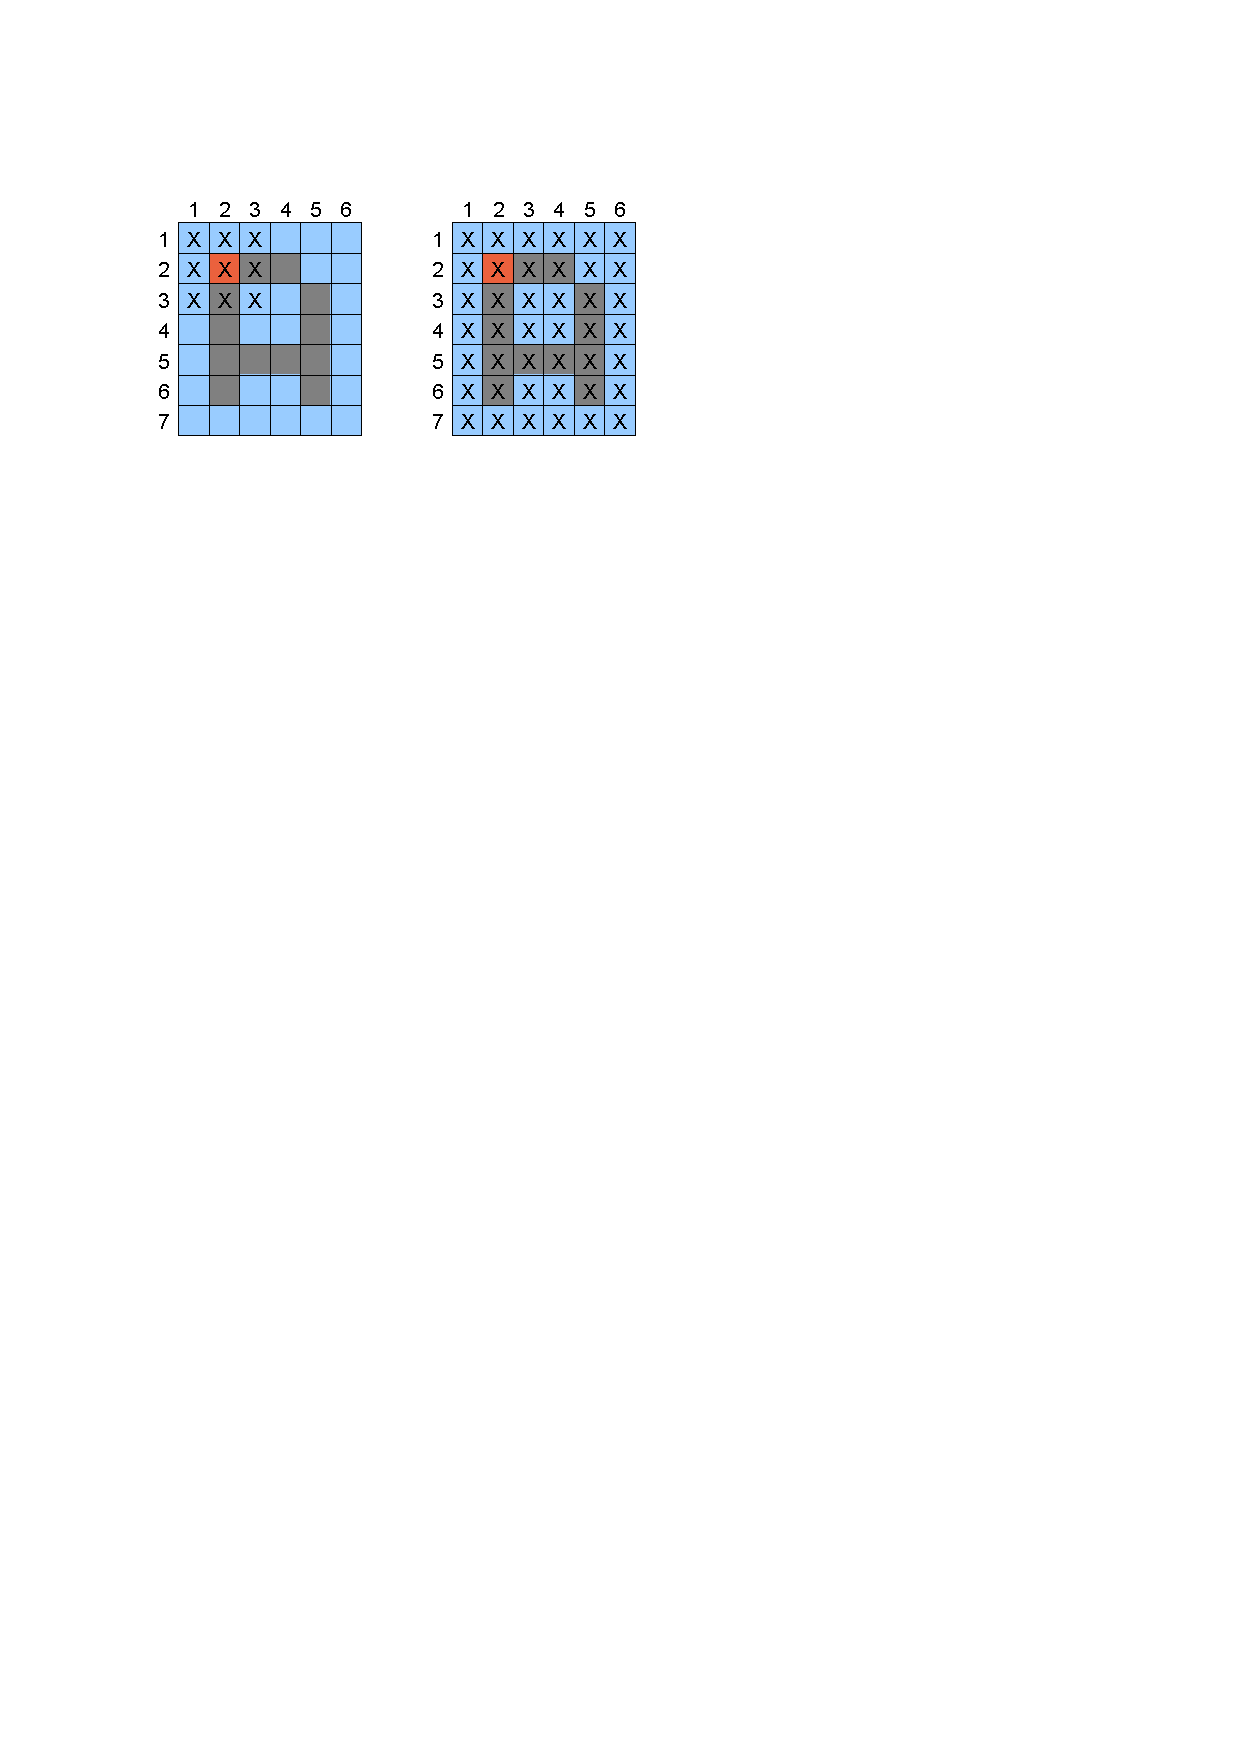
\includegraphics[]{local_nonlocal.pdf} %render with PDF
\caption{Differences between local (left) and non-local (right) processing. Red represents the pixel in focus, the X-s represent the pixels whose data the algorithm needs to access.}
\label{fig_local_nonlocal}
\end{center}
\end{figure}

The distinction between iterative and non-iterative algorithms is simpler: a non-iterative algorithm only processes the image a small, constant number of times to achieve the desired effect, whereas an iterative algorithm requires multiple passes, and often the output image of a previous pass becomes the input of the next pass. Observing the data requirements for what simply seems an iterative local algorithm, it is easy to see that even though the resulting values for pixels in the first pass only depend on their close neighborhood, from the second iteration on, those adjacent pixels have had their values adjusted according to their neighborhoods, which in turn are changed according to their neighbors and so on (see figure \ref{fig_local_iterative}). While the extent of this influence depends on the algorithm in question, the algorithm itself is - strictly speaking - non-local.

\begin{figure}[h]
\begin{center}
\includegraphics[scale=0.8]{local_iterative.eps} %TODO render with PDF
%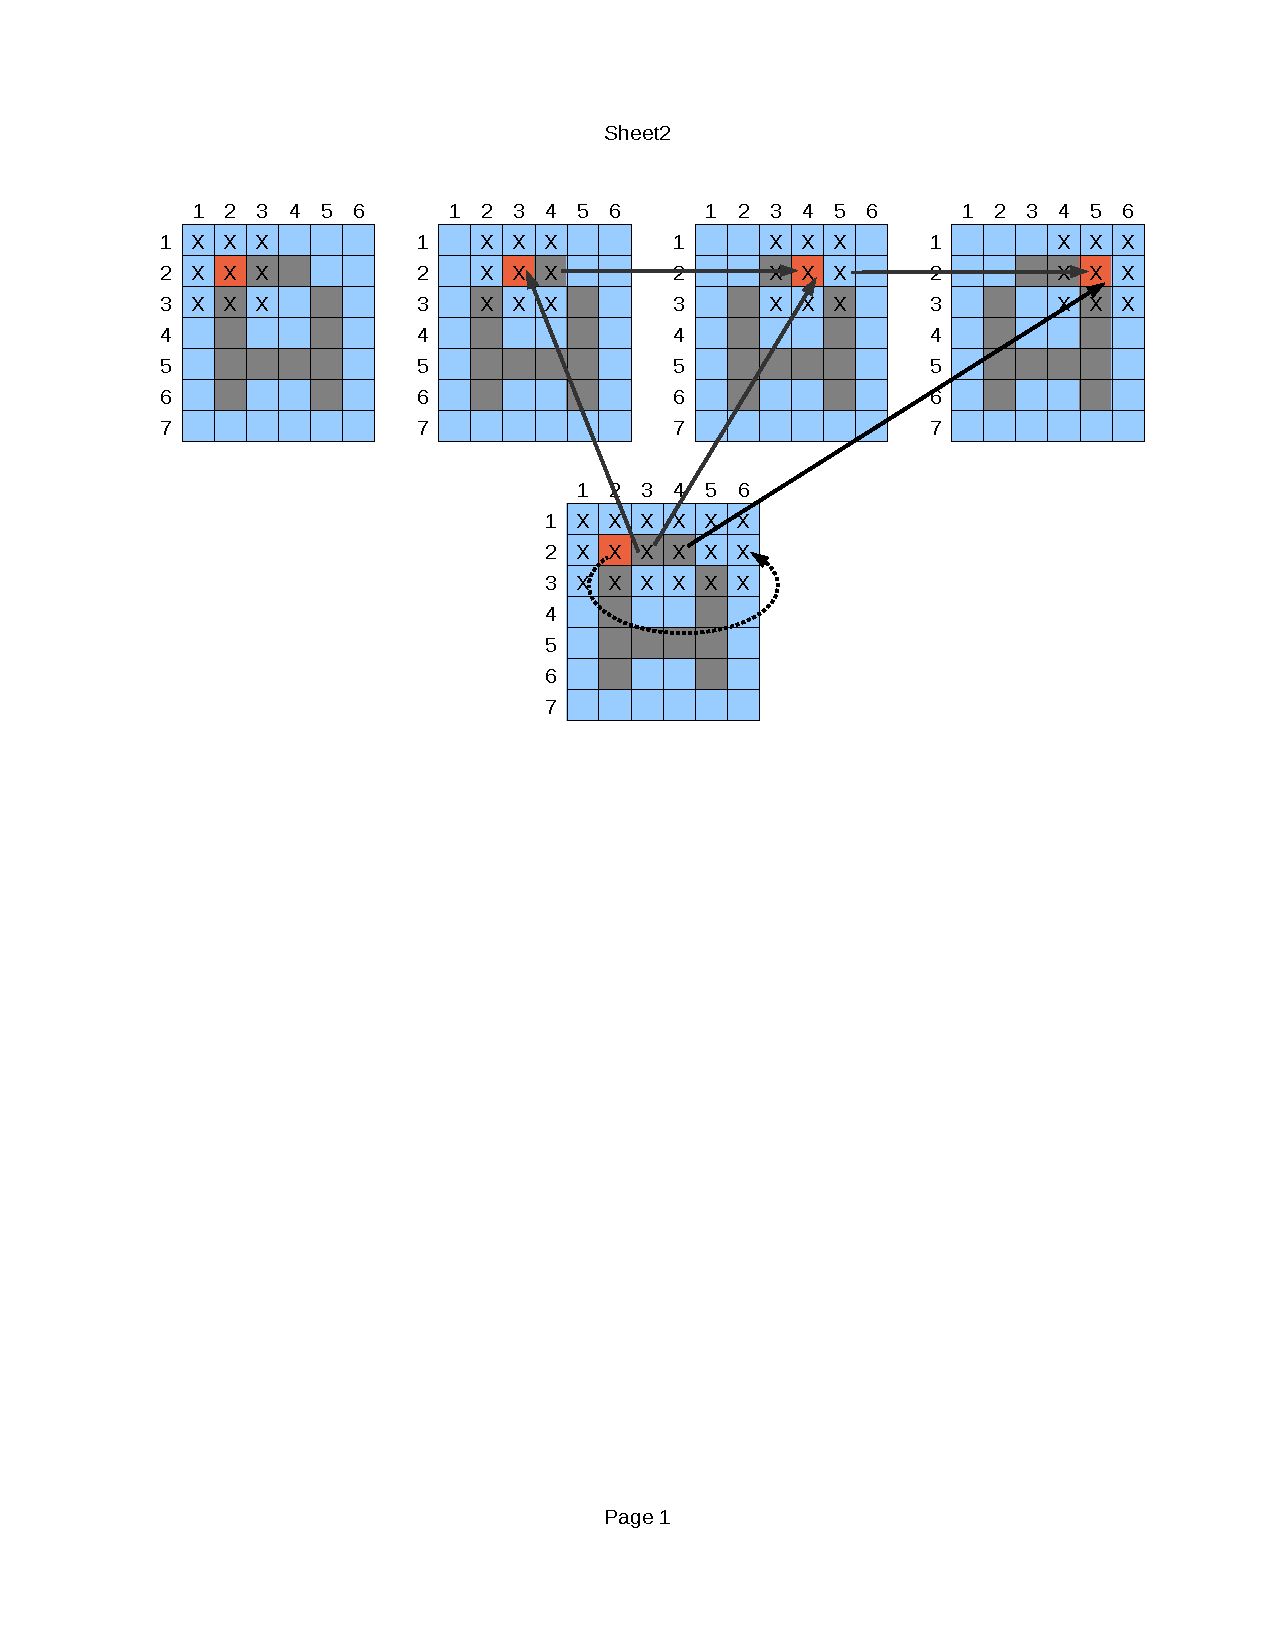
\includegraphics[scale=0.8]{local_iterative.pdf} %render with PDF
\caption{Illustration of the data requirements of iterative local processing. The top row represents first local computations of the first iteration. The diagram on the bottom shows the requirements at the start of the second iteration. Arrows encode a 'depends on' relationship: the value from which the arrow originates depends on the value the arrow is pointing at.}
\label{fig_local_iterative}
\end{center}
\end{figure}

Therefore, we can establish four classes of image processing problems: local, non-local, iterative local and iterative non-local. We can now look back at the example cases brought up previously and see what issues would arise if we attempted to parallelise local and non-local algorithms on these images.

In the first case of processing a 6.99 gigapixel image, it immediately becomes obvious that parallelising a non-local type of algorithm is going to be a non-trivial task, as we lack even the ability to store it in memory on regular computers. Even when assuming that the algorithm can continue to function if the input image is split to pieces, if communication is also required between the computers working on separate pieces, then there is a good chance that network speed will become a bottleneck and slow down the computation.

The second case, however, is far more suited for processing with the MapReduce model. Even though the total size of the data is several times bigger than in the previous case, since it consists of comparatively small images which easily fit into memory even when taking any algorithm-specific overhead into account. Moreover, because we do not have to split any images into pieces or worry about communication between worker computers, classification of the algorithms into the aforementioned four groups does not matter. Therefore, looking at the issues with regard to analysing this sort of data lets us make conclusions that apply to a wider range of problems. 

At this point it is important to note that we have so far silently assumed that all the algorithms we classify only require one image as an input. Speaking from the perspective of distributed processing, this means we assume that the algorithm only requires data from one image at a time. For example, with this clause we exclude any processing that needs to compare two or more images with each other from this discussion. The reason behind this will become clear further on in this text, as it is somewhat related to the implementation of the MapReduce model in Apache Hadoop and our approach to parallelising image processing tasks by dividing images into manageable pieces. Briefly and informally, it can be summarised as follows: if an algorithm requires access to more images than the local storage of the computer allows, communication between computers is needed. However, since a MapReduce calculation has only one step where the computing nodes exchange information, the only way to satisfy this need without resorting to another processing model is to run the MapReduce calculations themselves iteratively (note that when speaking about iterative image processing algorithms, I mean that all the iterations will be done within one MapReduce calculation). This, in turn, has been shown by Satish Srirama et al. to be very slow in actual performance, especially as the number of iterations increases \cite{srirama2012adapting}.

\subsection{Why use MapReduce?}

In the previous sections, I have presented some general analysis with regard to the general feasibility of using the MapReduce model of distributed computing to solve image processing tasks. In this part I will summarise the main motivation behind choosing MapReduce and it's implementation in the form of Apache Hadoop, and briefly outline alternative ways how one could approach distributed image processing.

First, what are the alternatives? Batch processing on the PC is feasible for only small amounts of data, and since only a part of this data fits into memory at given time, computation will suffer from a decrease in speed due to slow hard drive access. Trying to counter this by running the batch process on several computers simultaneously is a solution, but it creates a need for job monitoring, mechanisms for data distribution and means to ensure that the processing completes even when some computers experience failures during work. This is more or less exactly the problem that both Google MapReduce and Apache Hadoop were designed to solve. Another approach is treating the problem like a traditional large-scale computing task which requires specialised hardware and complex parallel programming. Cluster computers built on graphics processing units (GPU) are an example of this, and while maintaining a purpose-built computer cluster has been shown to be a working solution for many kinds of problems, it is interesting to know whether the same issues can be tackled with simpler and cheaper systems without much decrease in efficiency.

In conclusion, the main motivation behind using MapReduce (and more specifically Apache Hadoop) for image processing can be summed up in the following: as performing image processing is something that has already become a popular application of computing technology for an increasing amount of people, and because these tasks often require more processing capability than ordinary computers have, there is a need to turn towards distributed computing. On the other hand, since the MapReduce model implemented by Hadoop is currently one of the more popular such frameworks, it is a logical choice for trying to solve these processing issues, as it is freely available, provides a reliable platform for parallelising computation and does not have any requirements with regard to specialised hardware or software.

\chapter{Background}

In this chapter I will describe and summarise relevant work that has been done in the field of distributed image processing, then describe the MapReduce computing model with regard to Apache Hadoop and Hadoop Distributed Filesystem.

\section{Relevant work}

In order to gauge the relevance of addressing the problems brought up in the previous chapter, I will provide a brief overview of previous work sharing the themes of image processing and distributed computing in no particular order. 

In Web-Scale Computer Vision using MapReduce for Multimedia Data Mining \cite{White:2010:WCV:1814245.1814254}, Brandyn White et al. present a case study of classifying and clustering billions of regular images using MapReduce. No mention is made of average image dimensions or any issues with not being able to process certain images because of memory limitations. However, a way of pre-processing images for use in a sliding-window approach for object recognition is described. Therefore one can assume that in this approach, the size of images is not an issue, because the pre-processing phase cuts everything into a manageable size. The question still remains whether a sliding window approach is capable of recognizing any objects present in the image that do not easily fit into one analysis window, and whether the resource requirements for image classification and image processing are significantly different or not.

An Architecture for Distributed High Performance Video Processing in the Cloud \cite{Pereira:2010:ADH:1844768.1845374} by Rafael Pereira et al. outlines some of the limitations of the MapReduce model when dealing with high-speed video encoding, namely it's dependence on the NameNode as a single point of failure (however a fix is claimed at \cite{website:facebook_namenode_improvements}), and lack of possibility for generalization in order to suit the issue at hand. An alternative - optimized - implementation is proposed for providing a cloud-based IaaS (Infrastructure as a Service) solution. However, considering the advances of distributed computation technology within the past two years (the article was published in 2010) and the fact that the processing of large images was not touched upon, the problem posed in this work still remains.

A description of a MapReduce-based approach for nearest-neighbor clustering by Liu Ting et al. is presented in Clustering Billions of Images with Large Scale Nearest Neighbor Search \cite{citeulike:2631015}. This report focuses more on the technicalities of adapting a spill-tree based approach for use on multiple machines. Also, a way for compressing image information into smaller feature vectors is described. With regards to this thesis, again the focus is not so much on processing the images to attain some other result than something intermediate to be used in search and clustering.

In Parallel K-Means Clustering of Remote Sensing Images Based on MapReduce \cite{Lv:2010:PKC:1927661.1927687}, Lv Zhenhua et al. describe using the k-means algorithm in conjunction with MapReduce and satellite/aerophoto images in order to find different elements based on their color (i.e. separate trees from buildings). Not much is told about encountering and overcoming the issues of analyzing large images besides mentioning that a non-parallel approach was unable to process images larger than 1000x1000 pixels, and that the use of a MapReduce-based parallel processor required the conversion of TIFF files into a plaintext format.

Case Study of Scientific Data Processing on a Cloud Using Hadoop \cite{Zhang:2009:CSS:2127968.2128002} from Zhang Chen et al. describes the methods used for processing sequences of microscope images of live cells. The images and data in question are relatively small - 512x512 16-bit pixels, stored in folders measuring 90MB - there were some issues with regard to fitting into Hadoop DFS blocks which were solved by implementing custom InputFormat, InputSplit and RecordReader classes. No mention was made about the algorithm used to extract data from the images besides that it was written in MATLAB and MapReduce was only involved as a means distribute data and start the MATLAB scripts for processing.

Using Transaction Based Parallel Computing to Solve Image Processing and Computational Physics Problems \cite{trease08} by Harold Trease et al. describes the use of distributed computing with two examples - video processing/analysis and subsurface transport. The main focus is put on the specifications of the technology used (Apache Hadoop, PNNL MeDICI), whereas there is no information presented on how the image processing parts of the examples given were implemented.

In Distributed frameworks and parallel algorithms for processing large-scale geographic data \cite{Hawick:2003:DFP:958021.958024}, Kenneth Hawik et al. describe many problems and solutions with regard to processing large sets of geographic information systems' (commonly known as GIS) data in order to enable knowledge extraction. This article was published in 2003, so while some of the issues have disappeared due to the increase in computing power available to scientists, problems stemming from the ever-increasing amount of data generated by different types of monitoring technologies (such as ensuring distribution of data to computation nodes and storing big chunks of data in memory) still remain. Also, considering that the Amazon EC2 \cite{website:amazon_ec2} web service came online just in 2006, it is obvious that one can not make an apt comparison whether or not a MapReduce-based solution in 2012 is better or not for large-scale image processing than what was possible using grid technology in 2003.

A Scalable Image Processing Framework for gigapixel Mars and other celestial body  images \cite{5446706} by Mark Powell et al. describes the way NASA handles processing of celestial images captured by the Mars orbiter and rovers. Clear and concise descriptions are provided for the segmentation of gigapixel images into tiles, how these tiles are processed, and how the image processing framework handles scaling and works with distributed processing. The authors used the Kakadu JPEG2000 encoder and decoder along with the Kakadu Java Native Interface to develop their own processing suite. The software is proprietary and requires the purchase of a license to use.

Ultra-fast processing of gigapixel Tissue MicroArray images using high performance computing \cite{wang2011ult} by Yinhai Wang et al. talks about speeding up the analysis of Tissue MicroArray images by substituting human expert analysis for automated processing algorithms. While the images sizes processed were measured in gigapixels, the content of the image (scans of tissue microarrays) was easily segmented and there was no need to focus on being able to analyse all of the image at once. Furthermore, the work was all done on a specially built grid high performance computing platform with shared memory and storage, whereas this thesis is focused on performing processing on a Apache Hadoop cluster.

While the above shows that there has been a lot of work in this area the question remains whether (and how well) Hadoop is suited for large scale image processing tasks, because as evidenced by this brief overview, there are only a few cases where image processing has been done with MapReduce. 

\section{MapReduce}

MapReduce is a programming model developed by Google for processing and generating large datasets used in practice for many real-world tasks \cite{Dean:2008:MSD:1327452.1327492}. In this section, I will focus on describing the general philosophy and methodology behind this model, whereas the following part will describe in more detail one of the more popular implementations of the model - Hadoop - which is also used for all the practical applications featured in this work.

The basic idea behind MapReduce is based on the observation that a lot of processing tasks involving large amounts of data (i.e. terabytes or more) need to deal with the issues of distributing the data across a network of computers to ensure that the available memory, processor and storage are maximally utilised, and it would be easier if programmers could focus on writing the processing part that is actually different per task. To achieve this, the developer has to define only two functions - \textit{Map} and \textit{Reduce} - while everything else is handled by the implementation of the model. In reality, many more functionalities and parameters are provided for fine-tuning the system in order to help the model to better conform to the task at hand, however the core functionality can not be changed. Essentially, a MapReduce computation can be described as the following series of steps:

\begin{enumerate}
\item Input is read from disk, converted to Key-Value pairs.
\item The \textit{Map} function processes each pair separately, and outputs the result as any number of Key-Value pairs.
\item For each distinct key, the Reduce function processes all Key-Value pairs with that Key, and - similarly to Map - returns any number of Key-Value pairs.
\item Once all input pairs have been processed, the output of the Reduce function is then written to disk as Key-Value pairs. 
\end{enumerate}

It is important to note here that the MapReduce model simply specifies a very general structure with a focus on how data is put through calculation, but not what the different steps of the computation do with the data - it is expected that the user specifies this for all four steps. To illustrate this concept, a simple example of a MapReduce algorithm counting the occurrences of words in text documents is presented in figure \ref{fig_mapreduce}. In every step, the Key-Value pairs are processed independently, and therefore this processing can be distributed amongst a group of computers. Commonly, this is referred to as a \textit{cluster} and the individual computers that belong to it are called \textit{nodes}.

\begin{figure}[h]
\begin{center}
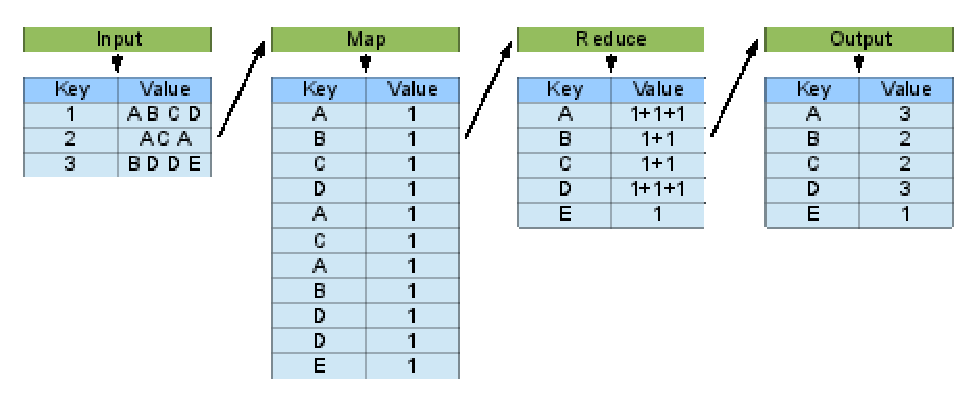
\includegraphics[scale=0.5]{mapreduce.eps} %TODO render with PDF
%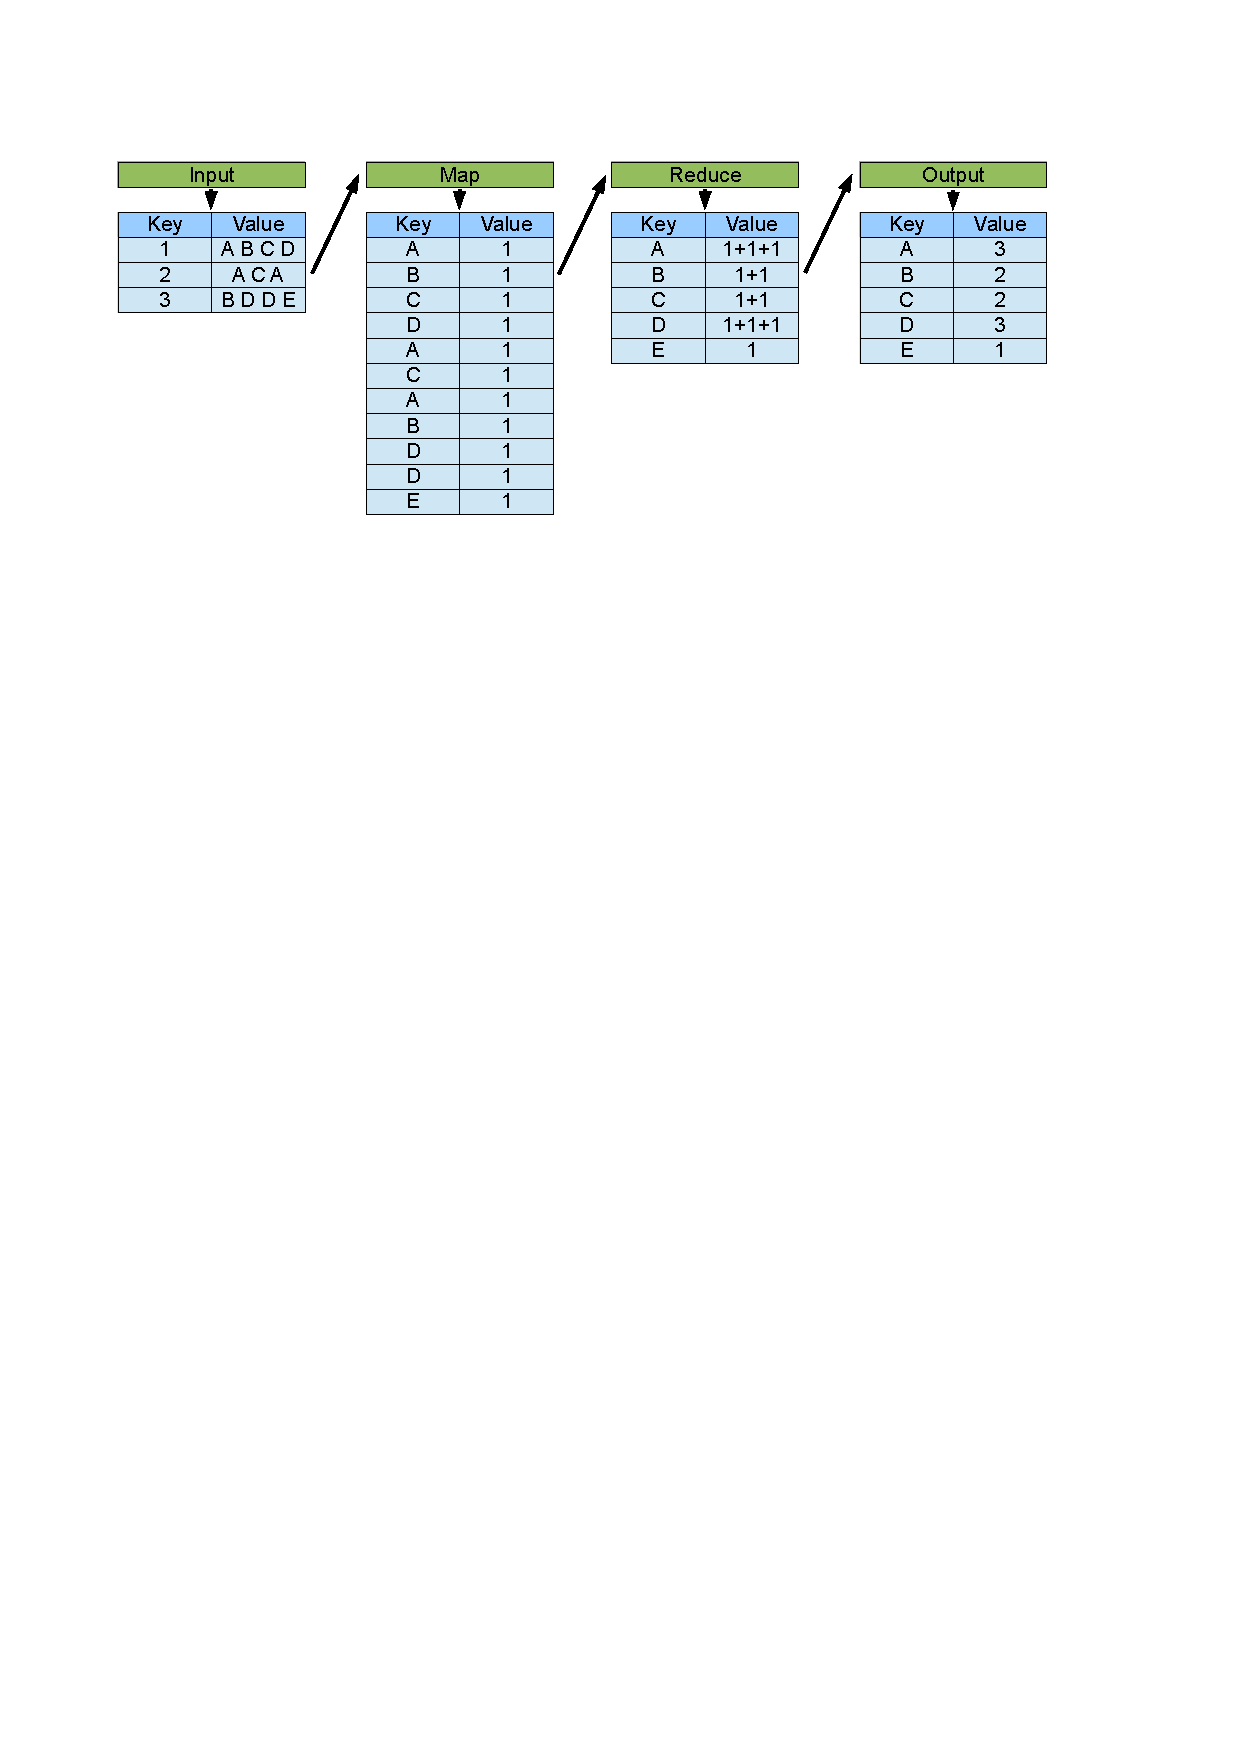
\includegraphics[scale=0.8]{mapreduce.pdf} %render with PDF
\caption{A simple example of the MapReduce computation model, inspired by the WordCount example provided in the Apache Hadoop Getting Started tutorial. A text file is first converted into pairs of line number and its content (Input), then the Map function splits these pairs further so that the reducer receives one pair per occurrence of a word. The objective of the Reduce function is then to count the individual occurrences and finally output the total per each distinct word.}
\label{fig_mapreduce}
\end{center}
\end{figure}

An important aspect of a MapReduce computation is also communication. Since every Map and Reduce task is designed to operate independently, communication between instances of the algorithm is not possible, except in the step where output from the Map phase is sent to Reduce. Here, all Key-Value pairs are grouped together by Key and the Reduce function can then process all Values together. However, short of starting another MapReduce computation whose input is the previous one's output (essentially making one MapReduce computation correspond to one iteration of the algorithm), there is no way to achieve communication between any given pair of Map or Reduce tasks. It is easy to see that if the start-up time of a MapReduce computation is significant, certain algorithms that need to take advantage of this sort of communication will suffer a decrease in performance.

Let us now analyse the adaptation of algorithms to the MapReduce model with regard to the four classes of image processing algorithms described earlier in this text. First, we see it is easy to adapt local non-iterative computations to this model. To do this, we simply define our Input step so that each image is represented by one Key-Value pair (in the case of large images, we split them to pieces beforehand). Then, the Map phase applies the algorithm, and results are returned by the Output step. Here, the Reduce step is defined as an identity function, meaning that it returns it's own input. The case is similar with local iterative algorithms, although - as discussed before - the approach of partitioning large images into manageable blocks will affect the results of the algorithm and may therefore be inapplicable. However, in some cases, this loss may be outweighed by gains in performance when compared to sequential processing.

Adapting both iterative and non-iterative non-local image processing algorithms to MapReduce is also straightforward when the images in question are small enough fit into memory. With bigger images, however, the issue becomes more complex, as this is the only scenario in which two processing tasks working on different pieces of the same image would need to communicate with each other. Due to these characteristics, these algorithms may require several MapReduce computations to complete and - as described above - can therefore be unsuitable for adaptation to the model, unless drastic changes are made. Due to these reasons and technical limitations of the Hadoop framework with regard to this sort of algorithms, I do not consider any such algorithms in this work.

\subsection{Apache Hadoop}
Hadoop is an open-source framework for distributed computing, written in Java and developed by the Apache Foundation and inspired by Google's MapReduce \cite{white2012hadoop}. It has been in development since 2005 and - at the time of writing this work - is one of the most popular freely available applications of it's kind. As the framework is already being used for large-scale data analysis tasks by many companies such as Facebook and Yahoo, and at the same time is easily adapted for use with any kind of hardware, ranging from a single computer to large data center, it is the best candidate for image processing on the MapReduce model. In the following, I will attempt to describe the basics of Hadoop's implementation in general and with regard to image processing. Since much of this topic is also covered in the Yahoo! Hadoop Tutorial, I am not going to explain the subjects of cluster set-up and writing MapReduce programs in much detail.

A typical Hadoop cluster consists of a master node and any number of computing nodes. The purpose of the master is to interact with users, monitor the status of the computing nodes, keep track of load balancing and handle various other background tasks. The computing nodes deal with processing and storing the data. The execution of a MapReduce program (alternatively, a \textit{MapReduce job}) can briefly be summed up in the following steps:

\begin{enumerate} 
\item The user uploads input data to the Hadoop Distributed File System (HDFS), which in turn distributes and stores it on the computing nodes.
\item The user starts the job by specifying the MapReduce program to execute along with input-output paths and other parameters.
\item The master node sends a copy of the program along with it's parameters to every computing node and starts the job.
\item Computing nodes start the Map phase first by processing data on their local storage, fetching more data from other nodes if necessary and possible (this decision is up to the master node).
\item After all Map tasks are finished, their output is sorted in a way, that for every distinct Key, a Reduce task processes all the pairs with that Key.
\item Once the Reduce phase is finished and it's output has been written back to HDFS, the user then retrieves the resulting data.
\end{enumerate}

In reality, this process is much more complicated due to procedures necessary for ensuring optimal performance and fault tolerance, among other things. A good example of this complexity is the time it takes for a MapReduce job to initialise: roughly 17 seconds. It is easy to see that this makes Hadoop unsuitable for any real-time processing and greatly reduces it's efficiency when considering approaches that involve iterating jobs. As Hadoop has hundreds of parameters for improving job efficiency, this subject is broad enough to warrant a study on its own. As discussed in previous parts, with regard to image processing we are mostly concerned with memory requirements and formatting the data to facilitate optimal processing.

Hadoop provides a fairly straightforward implementation of the MapReduce model. In order to write a complete a MapReduce job, a programmer has to specify the following things:

\begin{itemize}
\item A \textit{InputFormat} class, which handles reading data from disk and converting it to Key-Value pairs for the Map function. 
\item A \textit{Mapper} class, which contains the \textit{map} function that accepts the Key-Value pairs from \textit{InputFormat} and outputs Key-Value pairs for the Reduce function.
\item A \textit{Reducer} class with a \textit{reduce} function that accepts the Key-Value pairs output from the \textit{Mapper} class and returns Key-Value pairs.
\item A \textit{OutputFormat} class, which takes Key-Value pairs from the \textit{Reducer} and writes output to disk.
\end{itemize} 

Since the framework already comes with some basic implementations for all these classes, in very trivial cases, the programmer will just have to pick the ones that they need, and - assuming the Hadoop cluster is already set up - package the code into a Java Archive file (.jar), upload it to the master node and start the job. In reality, the Map and Reduce classes are usually custom-written for the task at hand, whereas customising InputFormat, OutputFormat and other helper classes is only necessary when the data is not readable using the pre-made classes. As Hadoop MapReduce jobs are themselves Java programs that can also be run independently (usually for testing purposes) without a previously set up computing cluster, and Hadoop places no restrictions with regard to the use of external libraries, the natural way to writing MapReduce jobs is using the Java programming language. However, the framework also provides a way to use functions written in essentially any language through the use of Hadoop Streaming and Pipes utilities. Furthermore, as demonstrated in the second use case scenario later in this work, the framework can simply be used to fulfill the role of distributing data, balancing loads and executing the scripts that handle the actual processing.

\subsubsection{Hadoop Distributed File System}

One of the integral parts of a Hadoop cluster is the Hadoop Distributed File System (HDFS). Inspired by the Google File System, it's purpose is to provide a fault-tolerant storage structure capable of holding large amounts of data, allow for fast access of said data, and provide a way for MapReduce to perform computations on the same location as the data \cite{ghemawat2003google,borthakur2007hadoop}. 

An important aspect of HDFS with regard to image processing is it's approach in storing files in blocks. Namely, while the block size of a regular file system - such as ext3 - is 1 to 8 kilobytes depending on the configuration, with HDFS, the default is 64 megabytes \cite{ext3}. There are two reasons for this design: as the blocks are written to physical storage in a contiguous manner, they can also be read with minimal disk seeking times, and because the file system is geared towards storing very large files, a larger block size ensures that storage of meta-data such as read/write permissions and physical locations of individual blocks creates less overhead. 

Block size is somewhat important with regard to processing images, since if an image that is too big is uploaded to HDFS, there is no guarantee that all of it's blocks would be stored in the same physical location. Since a Map or Reduce task would then have to retrieve all of it's blocks before processing, the idea behind executing tasks that are local with regard to the data is lost: the speed of reading input data now depends on the network. Therefore, in order to ensure optimal processing speed, images should fit inside the HDFS block size. This is not a problem with most regular images, as it is easily possible to configure the cluster with a block size of even 128 megabytes or more, however increasing this parameter past a certain point may not have the desired effects. Also, as discussed before, processing very large images sets considerable memory requirements to the computers. For these reasons, splitting large images into manageable parts is the best solution.

On the other hand, when dealing with a data-set of many small images, simply uploading them to HDFS results in the creation of a separate block for each file. Since a given Map or Reduce task operates so that it uses it's defined InputFormat to read data one block at a time, having many small blocks increases the overhead with regard to these operations. In these cases, it is standard practice to first store the data using a \textit{SequenceFile}. This file format is specifically geared towards storing Key-Value pairs which MapReduce operates on, and when loaded to HDFS, these files are automatically split into blocks, so that each block is independently readable. There is a caveat, however, with regard to the files that are located on the "edge" of the split. In order to illustrate this, I uploaded a SequenceFile with 3 images - 30 megabytes each - to HDFS with a configured block size of 50 megabytes. Quering the uploaded file with the Hadoop \textit{fsck} tool, I found that instead of writing the file as three blocks, each containing a full image, it was split into two blocks, so that one image ended up divided into two. This could negatively affect the performance of a job, since a Map or Reduce task would need to read both blocks to assemble the full image.

Most results presented in this thesis were attained with Hadoop version 0.20.2. While - at the time of writing this - there are several more current stable releases available, this choice was made because of the need to analyse the log files of completed MapReduce jobs using the Starfish Log Analyzer, developed by Herodotou et al. \cite{herodotou2011starfish}. To find out whether there are any drastic changes in performance in newer versions of Hadoop, some tests were also run with version 1.0.3, however no significant improvement was found.

%\section{Image processing and MapReduce}

%It is known that the MapReduce method places some restrictions on iterative parallel processing algorithms that require communication between computing nodes. Since the only step in a MapReduce job that contains any communication takes place when the mappers send data to reducers, all the algorithms whose parallelised implementations require more than one communication phase, require more than one MapReduce job to complete. Due to the overhead involved in starting jobs, this can lead to a huge increase in computation time, particularly for algorithms that require many iterations to complete, and therefore makes MapReduce less than ideal for performing this sort of processing.

%Fortunately, most image processing tasks involve doing many independent small-scale calculations in parallel. A good example of this is Gaussian blurring (smoothing), which transforms an input image by calculating a new value for every pixel based on it's neighbouring pixels. This procedure can be trivially parallelised since each calculation only requires the values of a small group of pixels in order to calculate the new value of the pixel in focus. In this case, the procedure requires only one step, so there is no need to worry about accommodating to iterations.

%Things get a bit more complicated once we attempt to use some sort of edge-detection heuristic in order to smooth only those regions in the image which are homogenous in colour, and preserve sharpness in the contours. A common approach here is to iteratively smooth the image, re-calculating the heuristic at every step. 

%TODO explain parallelisation by way of splitting the image into blocks, how to figure out the best block size analytically (take into account processing time, HDFS block size), overlap size etc.

%Description of different ways the MapReduce method has been used in conjunction with image processing libraries. Also some use cases.

%\chapter{Details of methodology}
%Descriptions on what was implemented, how it was implemented, problems encountered, and what has been done to solve these problems. If there were unsolvable problems, then how do these limit the applicability of the methodology in the real world and how to work around these limitations.

\chapter{Image processing with MapReduce in practice}

In this chapter, I will describe two example use cases inspired by real-world image processing problems. The first one deals with the application of an image processing pipeline geared towards object and text recognition on a photography data-set. In the second scenario, I describe running a local non-iterative algorithm on a single large image. In essence, these examples cover both general cases of large scale image processing: a data-set of regular images too big to process on a single computer, and an image with dimensions great enough to warrant distributed processing.

Since this thesis is aimed towards exploring the feasibility of distributed image processing using MapReduce, it should be noted the practical examples presented in the following text are meant to be a proof of concept, not robust and effective solutions for clearly defined problems. The following should be treated more as a broad description as to how to approach solving these sorts of problems using MapReduce and Hadoop.

\section{Processing a large data set of regular images}

In this section, we look at the subject of distributed image processing in the example case of a large data-set of regular-sized images. The data set consists of 48675 JPEG encoded images (a total of 265GB) taken across the span of 9 years at the Portus archaeological excavation site near Rome, Italy \cite{portusproject}. As the purpose of this data set is to provide a visual documentation of the activities of the project as thoroughly as possible, the subject matter of the photographs is rather varied: a random selection of images would probably contain examples of aerial photos, pictures of locations untouched by excavations and of areas already dug up and processed, among other things. In order to be able to use this in further work, it is necessary to organise it into a more logical structure and equip individual images with meta-data which can later be used to build indexes and allow searching. However, as the size of data grows, so does the amount of work necessary to file everything where it belongs.

Since traditionally there has been no easily-adaptable solution for doing this, the task of analysis and classification of all this information has fallen on humans. On the other hand, taking into account the advances in image processing techniques and general increase in available computing power, there may be ways to speed up this sort of processing, especially with regard to things that have in recent times been shown to be possible using computers, such as object and text recognition. From the perspective of a human, these are often trivial and repetitive tasks, and therefore should be automated. In the following, I will provide some examples of these images and outline some of the ways data- and image processing technologies could help solve these issues.

In order to proceed into specific approaches of extracting meaningful data, it is first important to look at some of the tasks which could be automated in the analysis and processing of this data-set. While methods of computer vision allow fairly complicated tasks to be solved, such as generating 3-dimensional models from single still images and utilising the internet for training object recognition models, in this case, our focus is much simpler \cite{sudo2009associative,saxena2008}. Discussing this matter with the archaeologists working with this data, and later condensing the list of issues that could feasibly be solved (both with regards to my understanding of the capabilities of current technology and the amount of resources at my disposal), I decided on the following:

\begin{itemize} 
\item Automatic tagging by meta-data.
\item Recognising the presence of certain objects of interest in the photographs.
\item Performing optical character recognition on photographed text.
\end{itemize} 

Before going into the specifics of solving these three tasks, it is important to note that since the aim of this thesis is to estimate the feasibility of using Apache Hadoop for large-scale image processing tasks, the solutions provided here should be viewed as proof-of-concept and be used only as starting points for more efficient realisations. However, with regard to providing some estimate as to whether using MapReduce for these sorts of problems, they should suffice.

\subsubsection{Classification by Exif meta-data and folder structure}

The first and probably the easiest way to approach the task of classifying and structuring a data set of this size is by taking advantage of all the information already present in the form of meta-data defined by the exchangeable image file format standard (Exif) \cite{japan2002jeita}. A simple example -already implemented in many pieces of photo management software - is grouping photos according to the creation date, which is a common meta-data tag. Moving further, it is a reasonable assumption that the initial step of sorting images has already taken place when the photographer moved the photos from the internal memory of the camera to a directory on their computer's file system. This means that even if only one image in a given subdirectory of the dataset has some specific tag-value pair (for instance tying the images to some specific geographic location), it could easily be added to all the other images in that subfolder, potentially reducing the workload of a human, who then has to only tag one image of a given group.

However, this only solves part of the problem, because we are also interested in grouping photos by geographic location and - ultimately - content. As the pictures are taken with cameras that do not possess a receiver that allows them to automatically tag images with geospatial coordinates, nor can they provide any useful description of photo content aside from the raw data itself, this information has to be extracted by either automatic or manual processing of image data. 

\subsubsection{Information extraction by object and text recognition}

Extracting Exif meta-data and making assumptions about the classification of images based on their location in the file system is connected with image processing only because the Exif standard deals with image files - this processing does not take the actual pixel data into account. However, as seen in figures \ref{archaeology_ex1} and \ref{archaeology_ex2}, there is definitely some information stored within this data that could be feasibly extracted programmatically. In the case of the first example - a photo of what appears to be a unearthed Roman coin - we would be interested in extracting the text on the paper and storing in within the Exif meta-data structure of that image. On the second image, the same sort of data is written by hand on a small blackboard, accompanied by markers to allow a human observer determine both the size of the object and the direction in which the photo was taken. It is important to note that this task is conceptually be split in two: trying to determine whether the objects are present in the image and if they are, attempting to extract the information they encode. The idea behind this approach is that even if we fail to automatically retrieve all the necessary data, knowledge that the image (or a certain part of the image) contains something of interest already helps narrow down the amount of images a human worker has to process.

\begin{center}
\begin{figure}[h]
\centering
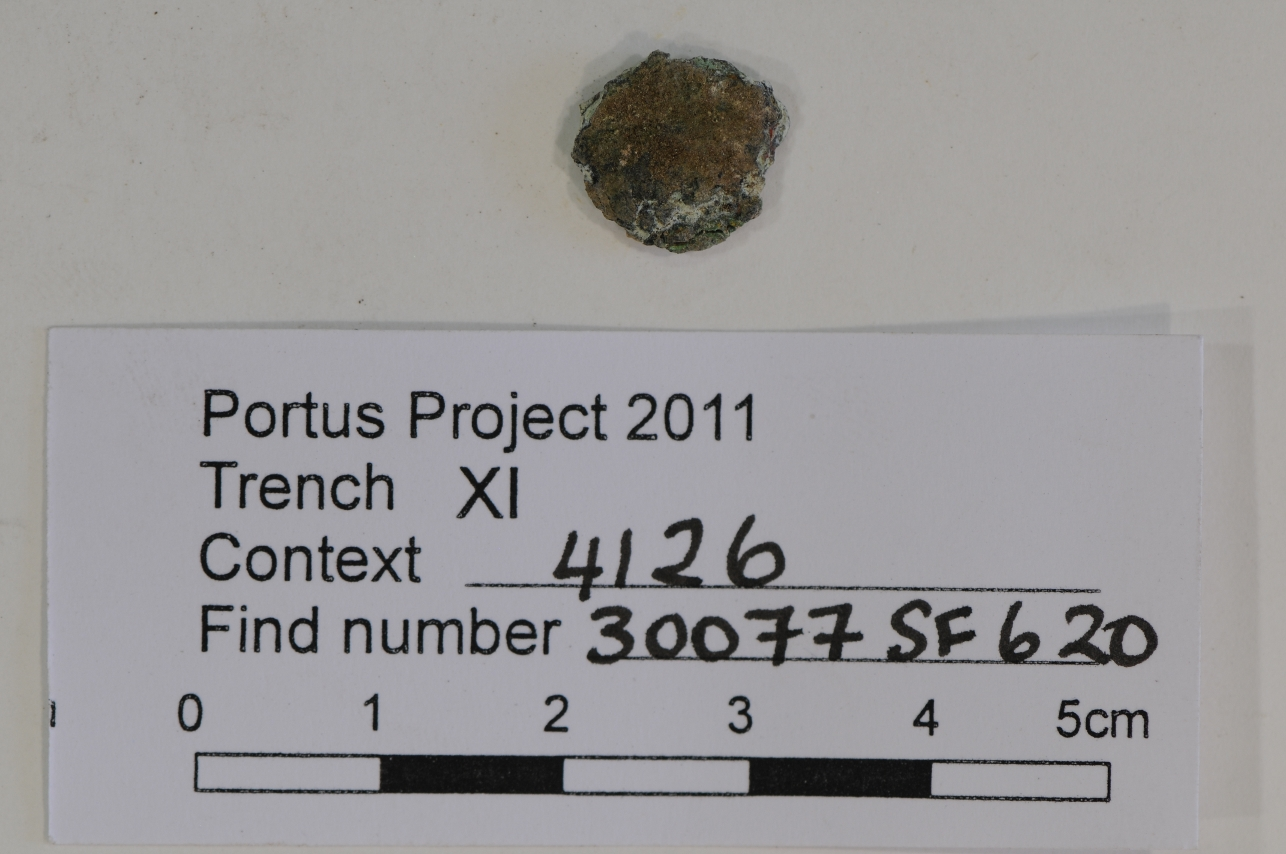
\includegraphics[scale=0.25]{archaeology_ex1.eps} %TODO render with PDF
\caption{A photo of an archaeological find with an accompanying description on a printed piece of paper. Images like this are good candidates for optical text recognition, because the text is clearly recognisable.}
\label{archaeology_ex1}
\end{figure}
\end{center}

\begin{center}
\begin{figure}[h]
\centering
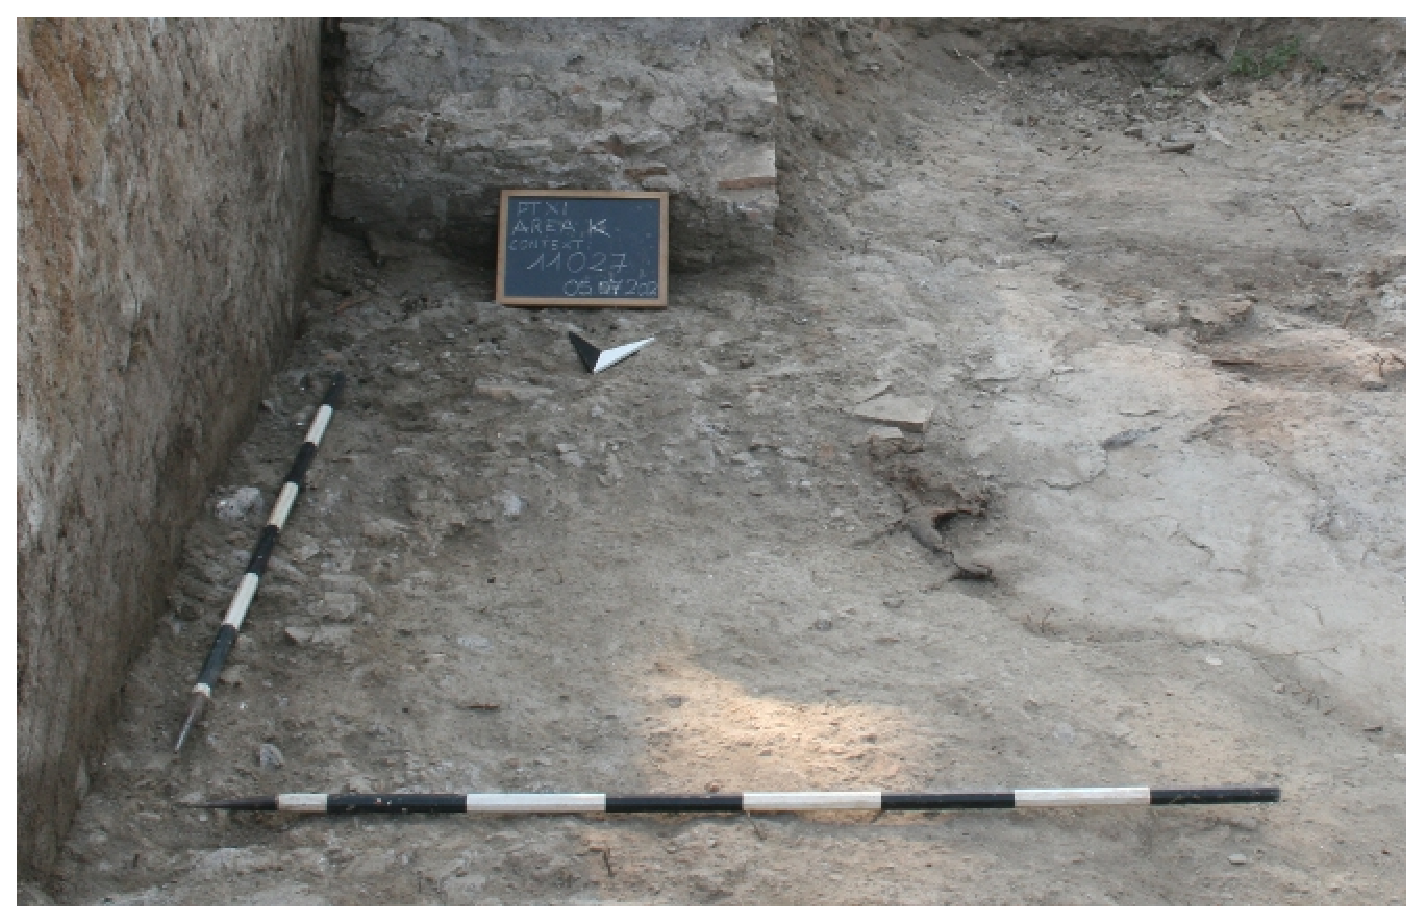
\includegraphics[scale=0.5]{archaeology_ex2.eps} %TODO render with PDF
\caption{A photo of an excavation site with a chalkboard and measuring artifacts. Extracting useful information from pictures like this is more difficult than is the case in figure \ref{archaeology_ex1}, because of recognition of handwritten text is complicated. }
\label{archaeology_ex2}
\end{figure}
\end{center}

\begin{center}
\begin{figure}[h]
\centering
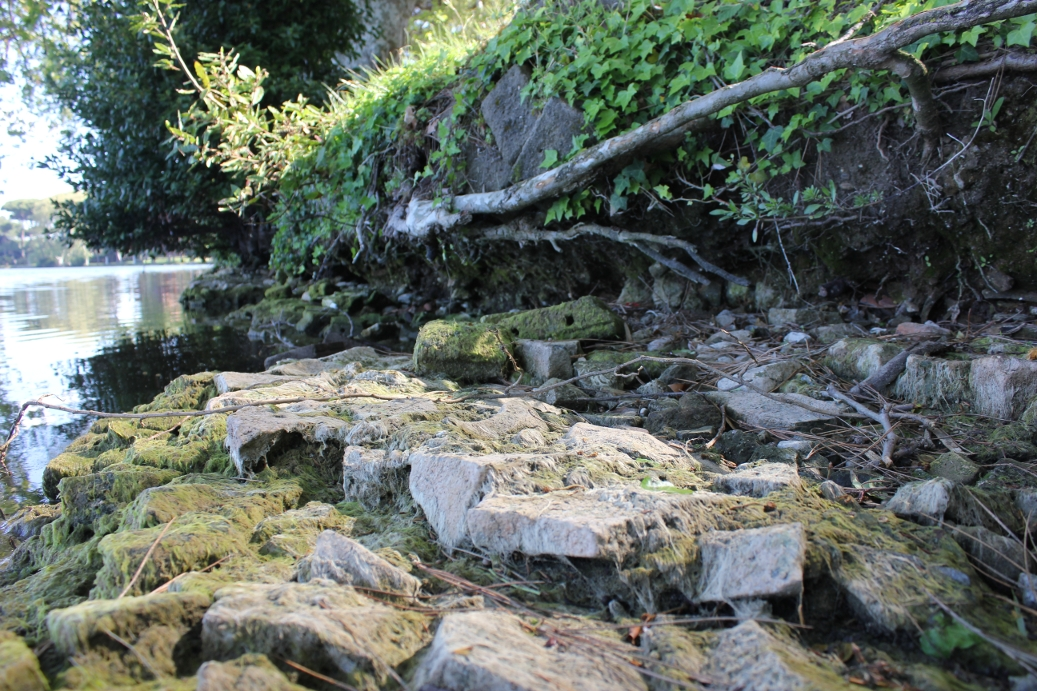
\includegraphics[scale=0.3]{archaeology_ex3.eps} %TODO render with PDF
\caption{A photo of random scenery. Extracting any useful information from here is practically impossible at the current state of technology. }
\label{archaeology_ex3}
\end{figure}
\end{center}

 %It is somewhat structured and some images are also tagged with meta-data using folder structures. However, the structuring is incomplete, as evidenced by many duplicate images and missing meta-data (which currently has to be manually added). The motivation behind applying distributed image processing on this data set is to find out whether it is possible to speed up the structuring process and extract some meta-data with minimal human interference.

%The downside of using this data set to illustrate the analysis of many small images using MapReduce is that since there is no ideally structured version of it to compare to, all efficiency statistics will be purely subjective. However the intent of this work is not to describe an effective meta-data extraction method, but rather analyse the suitability of MapReduce for this sort of task and discuss the issues (both solved and unsolved) encountered.

%TODO explain structure more

\subsubsection{Implementation in MapReduce}

As I mentioned before, in this case, the Hadoop framework is used mostly to ensure the distribution of data, whereas the processing itself is handled by a shell script which is executed from within the MapReduce job. This solution carries the additional overhead of having to write individual images back to the local file system of the computing nodes, as reading data straight from HDFS is non-trivial to implement in a shell script. However, this method allowed me to quickly develop a working distributed image processing pipeline, as I could simply chain together different existing tools without having to adapt anything into Java.
The first step in defining the MapReduce program for this task was figuring out the proper InputFormat to use. In this case, following the SequenceFile approach described earlier, I packaged the 48675 image files into 196 Key-Value collections, where the Key was set as the full path of the file with regard to the data-set, and Value as simply the contents of the file as a byte array.
The function of the Mapper in this case can be summarised to this: it writes the image to local storage, extracts Exif meta-data, starts the external shell script which runs the image through the processing pipeline, reads any output from the script, and returns all meta-data as Values. The Reducer simply sorts the data for a given image and formats it, so that the final output is written to disk in text format, and could further be treated as a table of comma separated values (CSV). For meta-data extraction, I used Drew Noakes' metadata-extractor \cite{metadataextractor}. In the following paragraphs, I will explain more about the function of the shell script, which does most of the heavy lifting with regard to image processing in this scenario.

\subsubsection{Image processing pipelie}

The main aim of the image processing pipeline is to provide a proof-of-concept solution to the tasks of recognising certain objects and extracting information by way of optical character recognition (OCR). As mentioned before, this is by no means a working solution that is ready to be applied in real world situations. However, a superficial analysis of the results suggests that, with some optimisation and tuning, it is suitable for extracting some information out of the data-set. The following is a rough description of each of the steps in the process:
\begin{enumerate}
\item The \textit{find\_obj} script performs object recognition and returns a list of matching pixel coordinates in the target image. In case of several pixels, the average is calculated. If no pixels were returned, halt processing.
\item Thresholding and labeling on the target image in order to convert it to a list of regions.
\item Erosion to eliminate regions that are too small.
\item Dilatation to bring the regions that remain back to their original size.
\item Calculate bounding boxes for all the remaining regions.
\item Based on the pixel coordinates from step 1, select the region that is located at these coordinates. If there is no region, halt processing.
\item The top left and bottom right pixel coordinate of the selected region specifies the area to extract from the target image.
\item Perform OCR using the Tesseract command line tool on the cropped part and write results into a text file.
\end{enumerate}

\begin{center}
\begin{figure}[h]
\centering
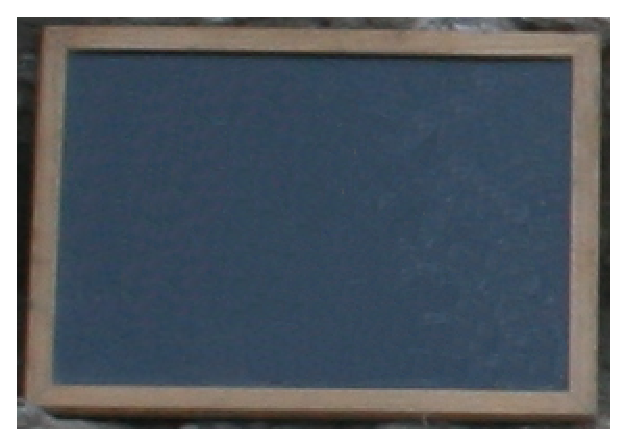
\includegraphics[scale=0.3]{box.eps} %TODO render with PDF
\caption{The query image used for object recognition.}
\label{box}
\end{figure}
\end{center}

In practice, I used this script to try and find the tablet shown in figure \ref{box}. If the tablet was found, the script attempts to extract the region containing it, and if that succeeds as well, it tries to recognise the handwritten text. For the first step, I adapted the \textit{find\_obj} example by Liu Liu from the Open Computer Vision library (OpenCV) \cite{opencv}, in order to retrieve the coordinates of matches in the target image. The script uses the library's implementation of Speed-Up Robust Feature (SURF) descriptor to find points in the target image that are similar to points in the query image \cite{bay2006surf}. An example can be seen in figure \ref{box_recognition}. Having found at least one matching point, we note that the image probably contains the object we are searching for. In this case, we move on to the next phase of processing: trying to extract the part of the image with the tablet.
To achieve this, I used a sequence of operations implemented as command line tools in the Pandore library \cite{pandore}. Processing starts by first segmenting the image two regions by pixel value (thresholding - figure \ref{fig_thresholding_small}) and assigning a different label to each separate region (labeling - figure \ref{fig_labeling_small}). After this, the script applies morphological processing in the form of erosion - a process which "erodes" the edges of regions and causes some of them to disappear (see figure \ref{fig_erosion_small}) - and dilatation, which is the reverse of erosion, in order to restore the size of the remaining regions. The final step in this phase is to calculate bounding boxes for the regions (figure \ref{fig_bounding_box_small}). Now, if a region is found to encompass the pixel coordinates returned by \textit{find\_obj}, the script extracts the area defined by this region from the original image.
If the script succeeded in extracting a region of the image, the Tesseract OCR tool is used to try and perform any text extraction \cite{tesseract}. 

%TODO box extraction by Python script and ImageMagick convert functions \cite{imagemagick, python}

\begin{center}
\begin{figure}[h]
\centering
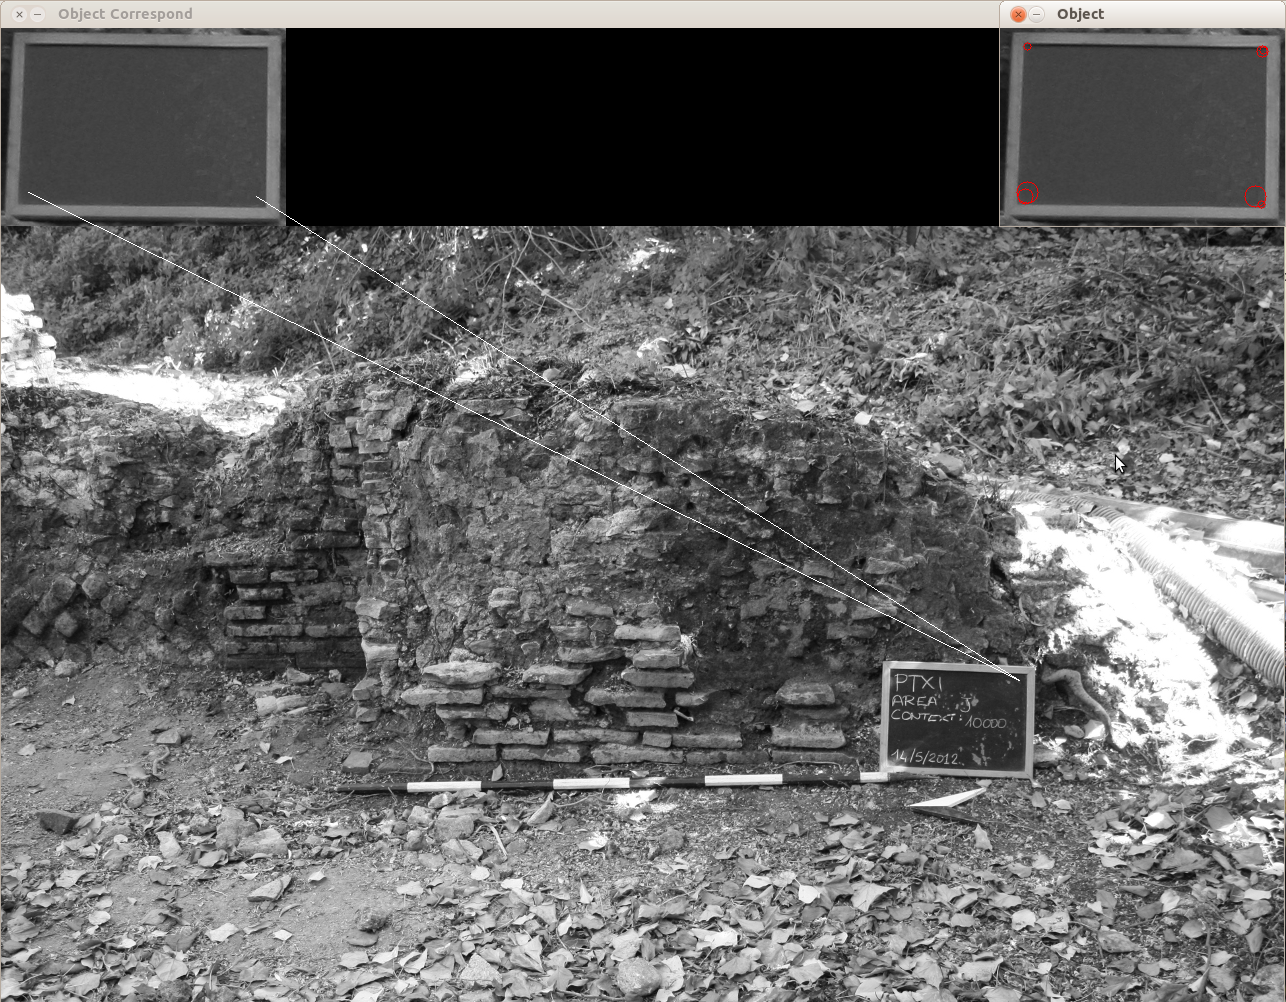
\includegraphics[scale=0.3]{box_recognition.eps} %TODO render with PDF
\caption{Screenshot of the original \textit{find\_obj} from OpenCV examples used to recognise the tablet from the photo.}
\label{box_recognition}
\end{figure}
\end{center}

%\begin{center}
\begin{figure}[h]
\begin{subfigure}{.5\textwidth}
  \centering
  
\includegraphics[scale=0.27]{input_small.eps} %TODO render with PDF
	\caption{}
	\label{fig_input_small}  
\end{subfigure}%
\begin{subfigure}{.5\textwidth}
  \centering
  
\includegraphics[scale=0.27]{thresholding_small.eps} %TODO render with PDF
	\caption{}
	\label{fig_thresholding_small}   
\end{subfigure}
\\
\\
\begin{subfigure}{.5\textwidth}
  \centering
  
\includegraphics[scale=0.27]{labeling_small.eps} %TODO render with PDF
	\caption{}
	\label{fig_labeling_small}
\end{subfigure}%
\begin{subfigure}{.5\textwidth}
  \centering
  
\includegraphics[scale=0.27]{erosion_small.eps} %TODO render with PDF
  \caption{}
	\label{fig_erosion_small}
\end{subfigure}
\\
\\
\begin{subfigure}{.5\textwidth}
  \centering
  
\includegraphics[scale=0.27]{dilatation_small.eps} %TODO render with PDF
	\caption{}
	\label{fig_dilatation_small}
\end{subfigure}%
\begin{subfigure}{.5\textwidth}
  \centering
  
\includegraphics[scale=0.27]{bounding_box_small.eps} %TODO render with PDF
	\caption{}
	\label{fig_bounding_box_small}
\end{subfigure}
\\
\begin{subfigure}{1.0\textwidth}
  \centering
  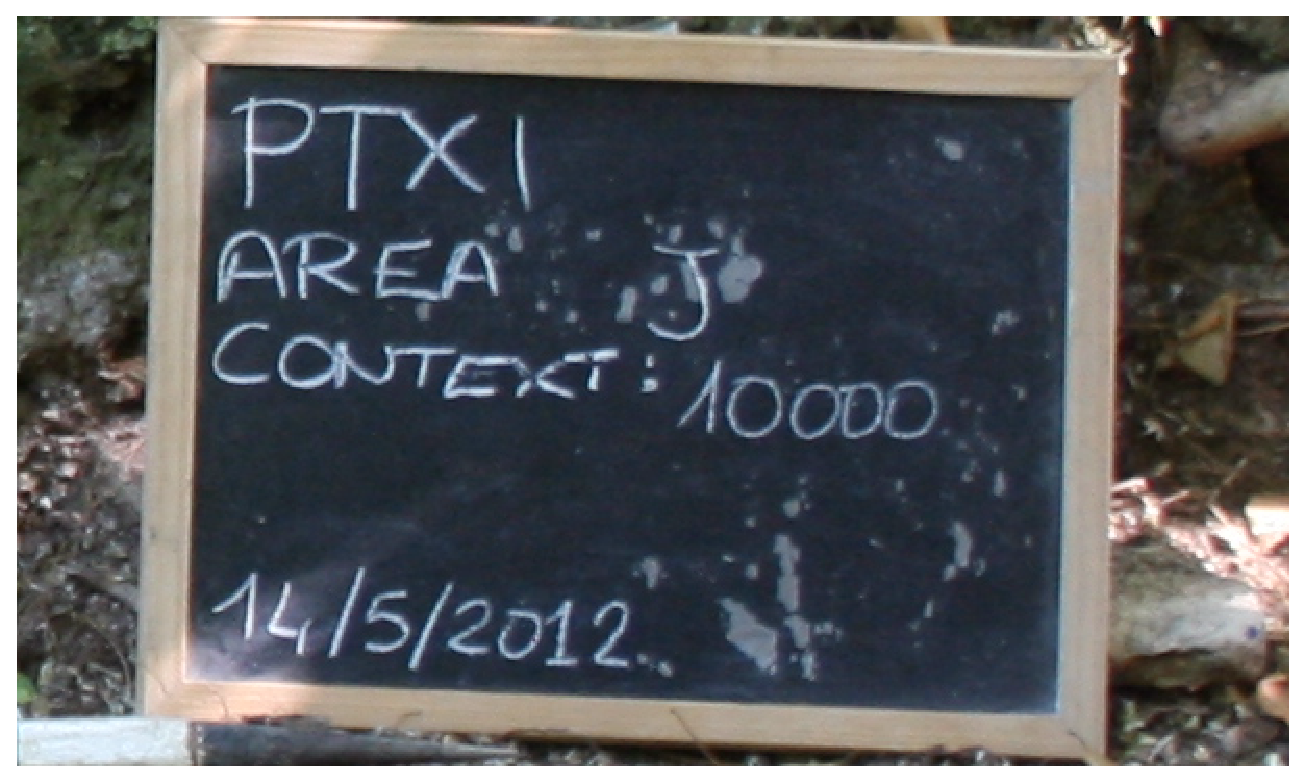
\includegraphics[scale=0.3]{box_extracted.eps} %TODO render with PDF
  \caption{}
	\label{fig_box_extracted_small}
\end{subfigure}
\caption{Step-by-step example of the extracting the region containing the tablet.}
\label{fig_pipeline_examples}
\end{figure}
%\end{center}

\subsection{Results}

Processing the data-set with a 16-node Hadoop cluster running version 0.20.2 took \textbf{12,5 hours} ($\sim0.9$ seconds per image on average), with 8 worker nodes, this number increased to \textbf{24,2} ($\sim1.8$ seconds per image). Since this trend probably continues as the size of the cluster decreases, we can assume a total execution time of roughly 194 hours (at $\sim14$ seconds per image) - roughly 8 days - to process all 48675 photos in the data-set.

\section{Processing a large image using a local non-iterative algorithm}

In this section, I will describe a practical application of distributed image processing in the scenario of applying a local non-iterative algorithm on a image with large spatial dimensions. The rest of this section is structured as follows: first, a description of the image itself and the motivation behind the task. Further on, I will outline the divide-and-conquer approach used in splitting the image into manageable pieces, briefly describe the specifics of the MapReduce implementation of the algorithm and how it's performance was measured and compared with it's non-distributed (sequential) counterpart.

\subsection{Description of the data and use case}

As already briefly mentioned in the introduction of this work, the image in question is a photograph taken by a microscope, with a width and height of 86273 and 81025 pixels, respectively, and stored in a GeoTIFF container \cite{mahammad2003geotiff}. The subject matter is a group of cells, and the objective of image processing in this case is to somehow programmatically count the number of nuclei in the image. One probable step in such an image processing computation is to smooth colours in the image while accenting the edges in order to allow for more easier detection of nuclei. The fast O(1) bilateral filter algorithm is a local, non-iterative way of accomplishing this, and therefore a good candidate for applying on the image even when it has been partitioned in order to fit into memory of all the nodes in the Hadoop cluster.

\begin{center}
\begin{figure}[h]
\begin{subfigure}{.5\textwidth}
  \centering
  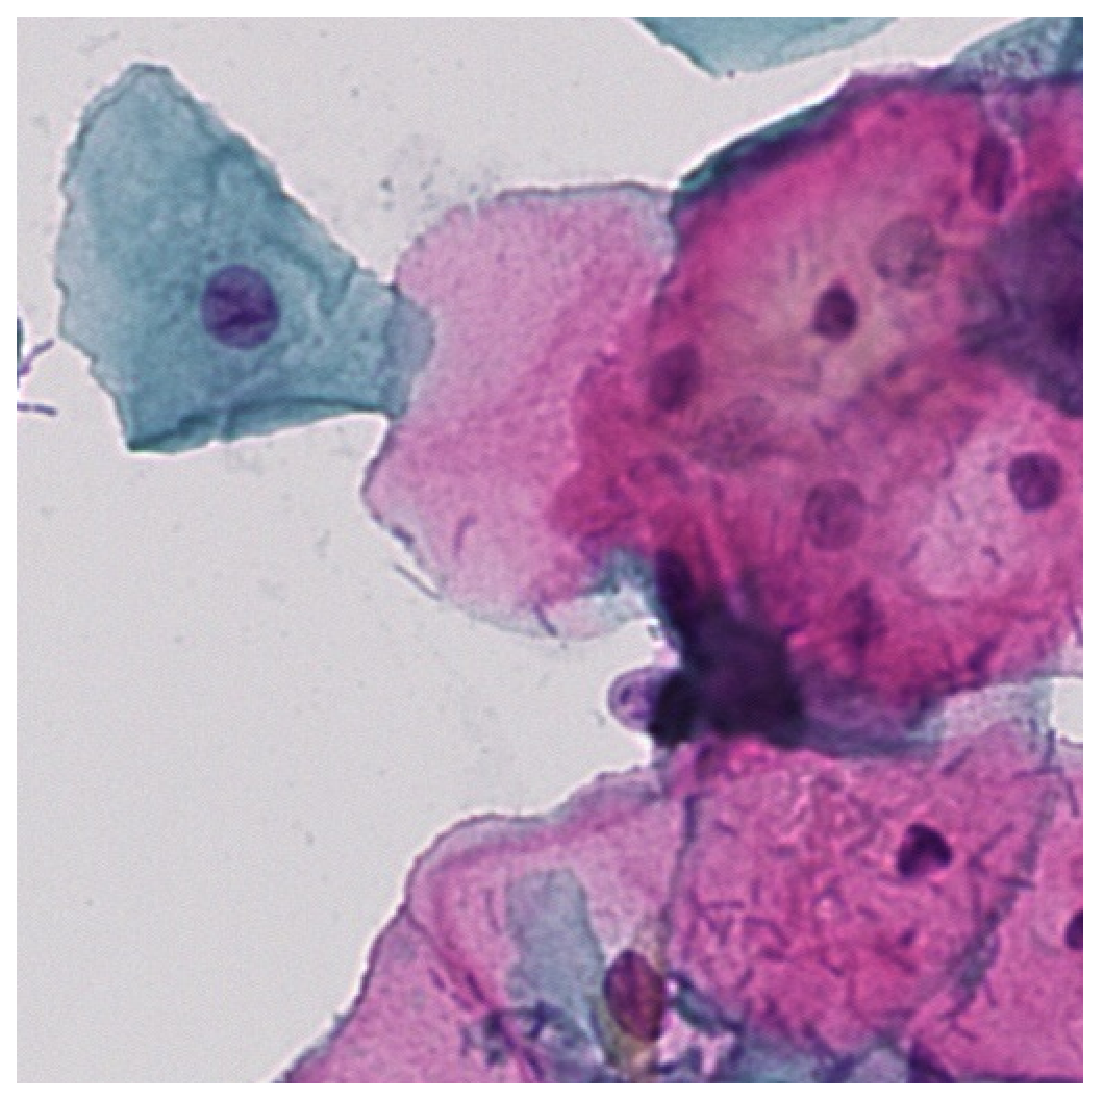
\includegraphics[scale=0.3]{microscope.eps} %TODO render with PDF
  %\caption{Regular image}
  %\label{fig:sub1}
\end{subfigure}%
\begin{subfigure}{.5\textwidth}
  \centering
  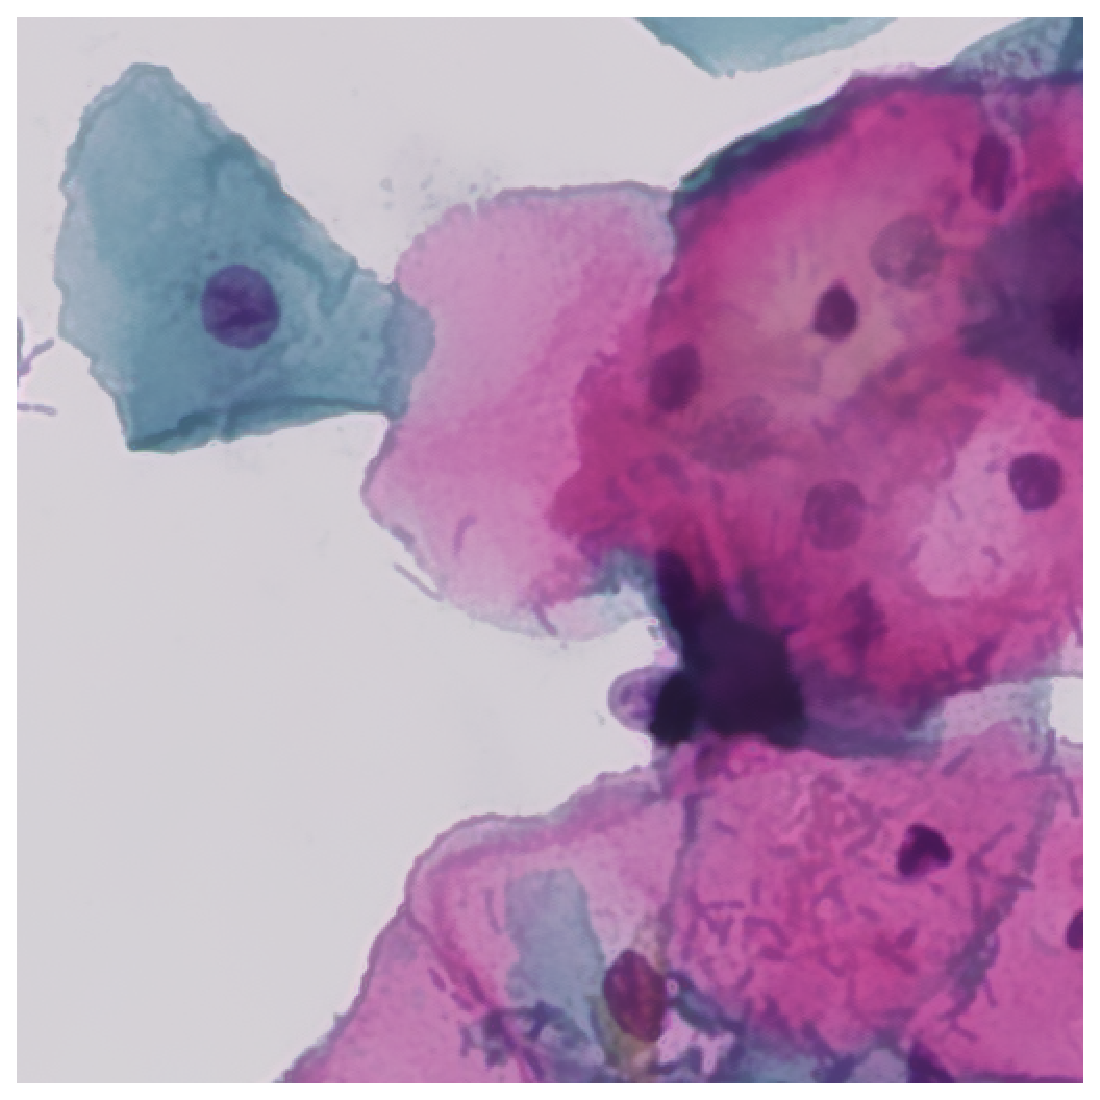
\includegraphics[scale=0.3]{microscope_bf_10_10.eps} %TODO render with PDF
  %\caption{A subfigure}
  %\label{fig:sub2}
\end{subfigure}
\caption{On the left - a 512 by 512 pixel detail of the microscope image. On the right - results of fast O(1) bilateral filtering with $\sigma_s, \sigma_r$ = 10. The dark spots are the nuclei of the cells, which are now more defined on the processed image, allowing for easier object recognition.}
\label{fig_microscope}
\end{figure}
\end{center}

\subsection{Bilateral Filter}

In the context of this thesis, I will refer to the bilateral filter as a smoothing filter that attempts to preserve edges while reducing noise in the image. It has previously been described by Aurich and Weule, Tomasi and Manduchi, and Smith and Brady \cite{aurich1995non,smith1997susan,tomasi1998bilateral}. This section will describe both the naive and optimised implementations with regard to performance and resource requirements and provide a brief overview of it's common uses. The following descriptions are adapted from course notes by Paris et al. \cite{bf_course}. In the interests of simplicity and also due to differences between real-world implementations of these algorithms with regard to processing images with more than one color channel, the formulations here will apply only to images with a single number as the pixel value (i.e. monochrome images). In general, however, it can be assumed that given a multichannel image, the algorithm will simply process each channel separately.

%\subsubsection{Image processing}

As already mentioned in the preceding text, I will restrict the focus of this thesis to the field of image processing to two-dimensional color images. The following will not be a description of how images are acquired through the use of scanning or digital cameras, therefore it is assumed here that the reader is familiar with the notions of pixels, 2-dimensional coordinate notation and representing color using red, green and blue values. Therefore I will start with the following formal definition: I consider the image $I$ with width $x$ and height $y$ as a collection of pixels $p$, such that

\begin{center}
$I = \{ \, p_{i,j} | \, i \in [1,x], \, j \in [1,y] \, \}$, and

$p_{i,j} = (r_{i,j}, g_{i,j}, b_{i,j})$,
\end{center}
where $r_{i,j}$, $g_{i,j}$ and $b_{i,j}$ are respectively the red, green and blue values of the pixel at $x$-coordinate $i$ and $y$-coordinate $j$. From this definition it is more or less straightforward to estimate the minimal memory requirements for storing an image with known dimensions when the programming language and data type for storing individual color values is also chosen. Since this thesis deals with Java, and image processing algorithms tend to prefer floating point values (which are 32 bits in Java) in the interests of precision, we can estimate the memory consumption $M$ of an image with dimensions $x$ and $y$ as follows:

\begin{center} 
$M = x * y * 3 * 32$ bits.
\end{center}

As image processing algorithms tend to operate on uncompressed images, using this sort of calculations provides a way of estimating the memory requirements from the time complexity of the processing tasks. Therefore the size of compressed the image file (for example JPEG or PNG) is only very loosely correlated with the time it takes to process that image, as the efficiency of compression algorithms depends on the information content of the image itself, whereas the estimation method described above only takes into account the spatial dimensions of the image.

\subsubsection{Gaussian blur}

One of the simplest local algorithms in image processing is Gaussian blur (also known as Gaussian smoothing). It's most common application is noise reduction. An example can be seen in figure \ref{fig_gaussian_blur}. The bilateral filter algorithm described later on in this thesis is an improvement of Gaussian blur with regard to edge-preservation capability. The following is a formal description of the algorithm:

\begin{center}
\begin{algorithm}[h]
	\KwData{$I$ - input image, $O$ - output image, $\sigma$ - filter range, $h$ - height of the input image, $w$ - width of the input image}
	\For{$x = 1, 2, ... w$}{
		\For{$y = 1, 2, ... h$}{
			$O(x,y) = 0$

			\For{$x_\sigma = x-\sigma ... x+\sigma$}{
				\For{$y_\sigma = y-\sigma ... y+\sigma$}{
					$O(x,y) += I(x_\sigma, y_\sigma)G_\sigma(\| (x_\sigma, y_\sigma)-(x, y) \|)$
				}
			}
		}
	}
\end{algorithm}
\end{center}

Here, $I(x,y)$ and $O(x,y)$ signify pixels of input and output images at width and height coordinates $x$ and $y$ respectively, $\| (x_\sigma, y_\sigma)-(x, y) \|$ represents the distance between the pixel being processed and the pixel at $(x_\sigma, y_\sigma)$. $G_\sigma(x)$ is the Gaussian function
\begin{center}
$G_\sigma(x) = \frac{1}{2\pi\sigma^2} \exp(-\frac{x^2}{2\sigma^2})$.
\end{center}

TODO verify if the above is correct.

Essentially, what happens to each pixel during the course of this algorithm, is that their values are re-calculated as a weighted sum of their neighboring pixels, and $\sigma$ specifies the range of this neighborhood. This is best visualised by thinking of pixels as cells and the image as the table - the $\sigma$-neighborhood of pixel $I(x,y)$ then is the group of cells extending $\sigma$ rows above and below, and $\sigma$ columns before and after the cell in focus (see figure \ref{fig_gaussian_blur}). Due to the characteristics of Gaussian distribution, as the distance $\| (x_\sigma, y_\sigma)-(x, y) \|$ between pixels increases, the weight decreases. This means that pixels further away contribute less to the new value of the pixel currently in focus, and pixels outside the $\sigma$-neighborhood of the pixel do not affect it's value at all. It is important to note here that the actual values of the pixels do not affect the calculations of the weights at all, and the $G_\sigma(x)$ can be pre-calculated as a matrix of weights, bringing the time complexity of the algorithm to $O(n)$, where $n$ is the amount of pixels in the image.

%\begin{center}
\begin{figure}[h]
\begin{subfigure}{.5\textwidth}
  \centering
  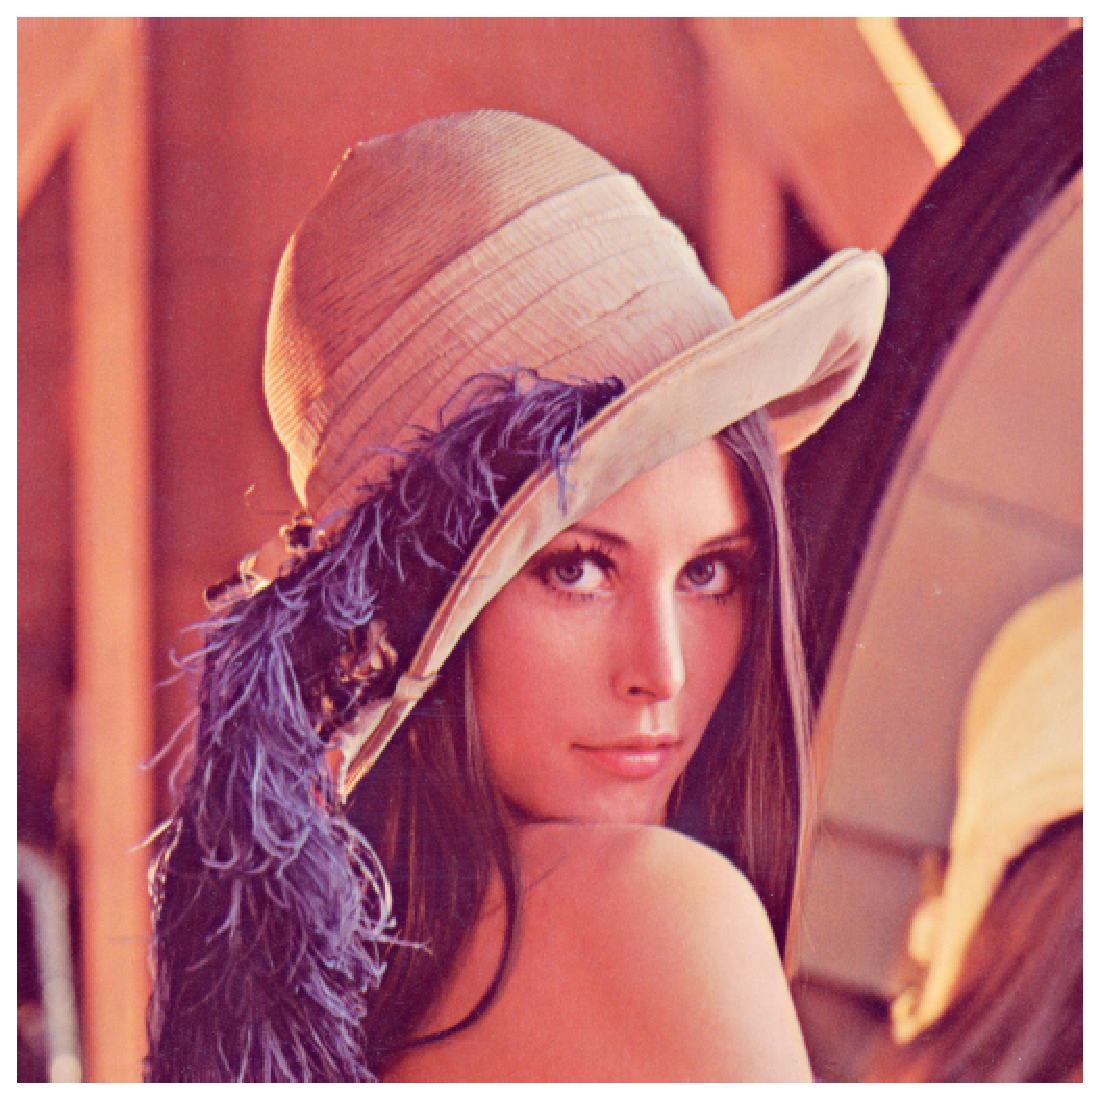
\includegraphics[scale=0.35]{Lenna.eps} %TODO render with PDF
  %\caption{Regular image}
  %\label{fig:sub1}
\end{subfigure}%
\begin{subfigure}{.5\textwidth}
  \centering
  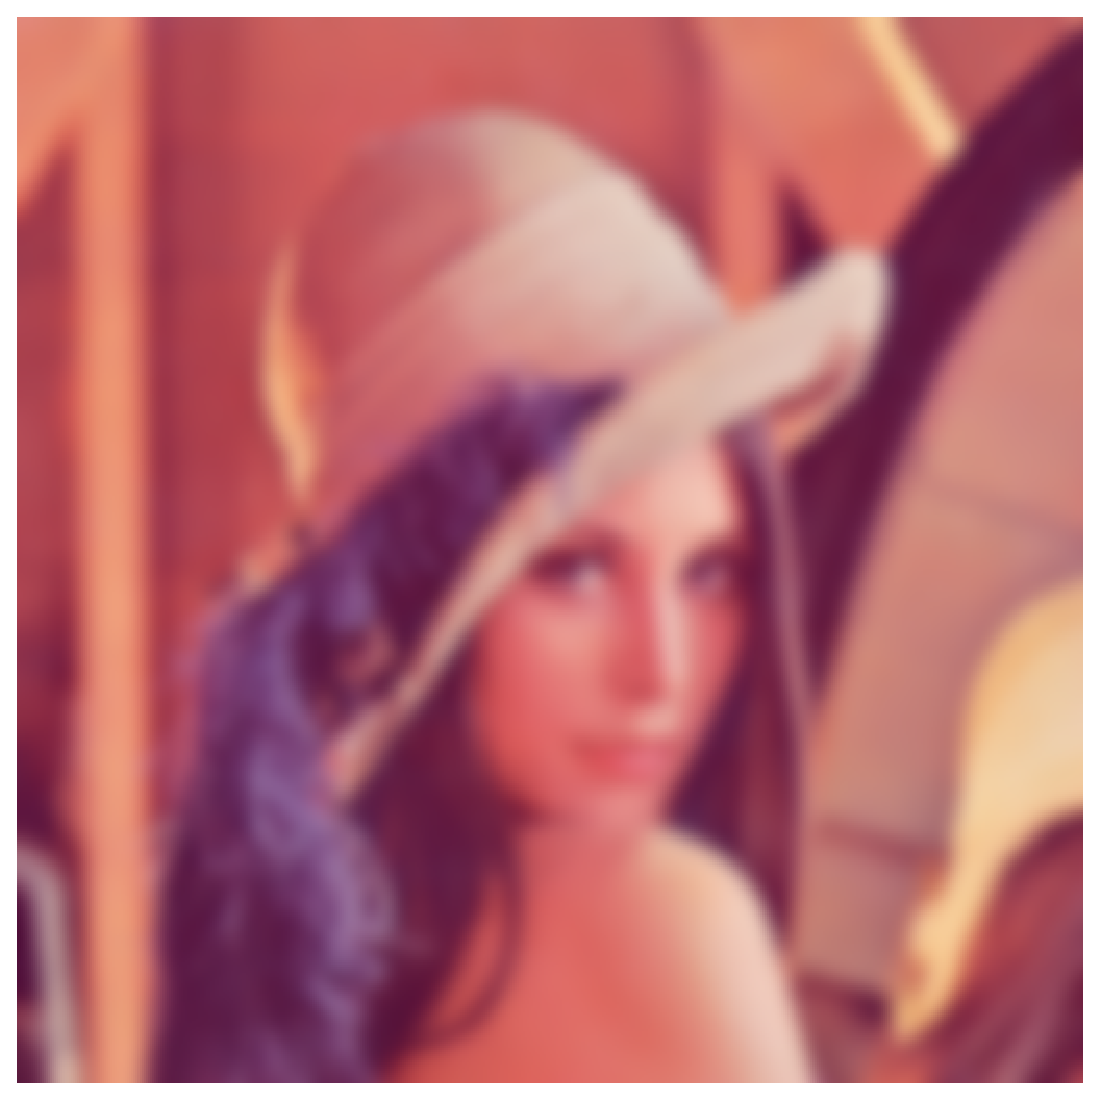
\includegraphics[scale=0.35]{Lenna_gaussian_10px.eps} %TODO render with PDF
  %\caption{A subfigure}
  %\label{fig:sub2}
\end{subfigure}
\\
\\
\begin{subfigure}{1.0\textwidth}
  \centering
	%\begin{center}
  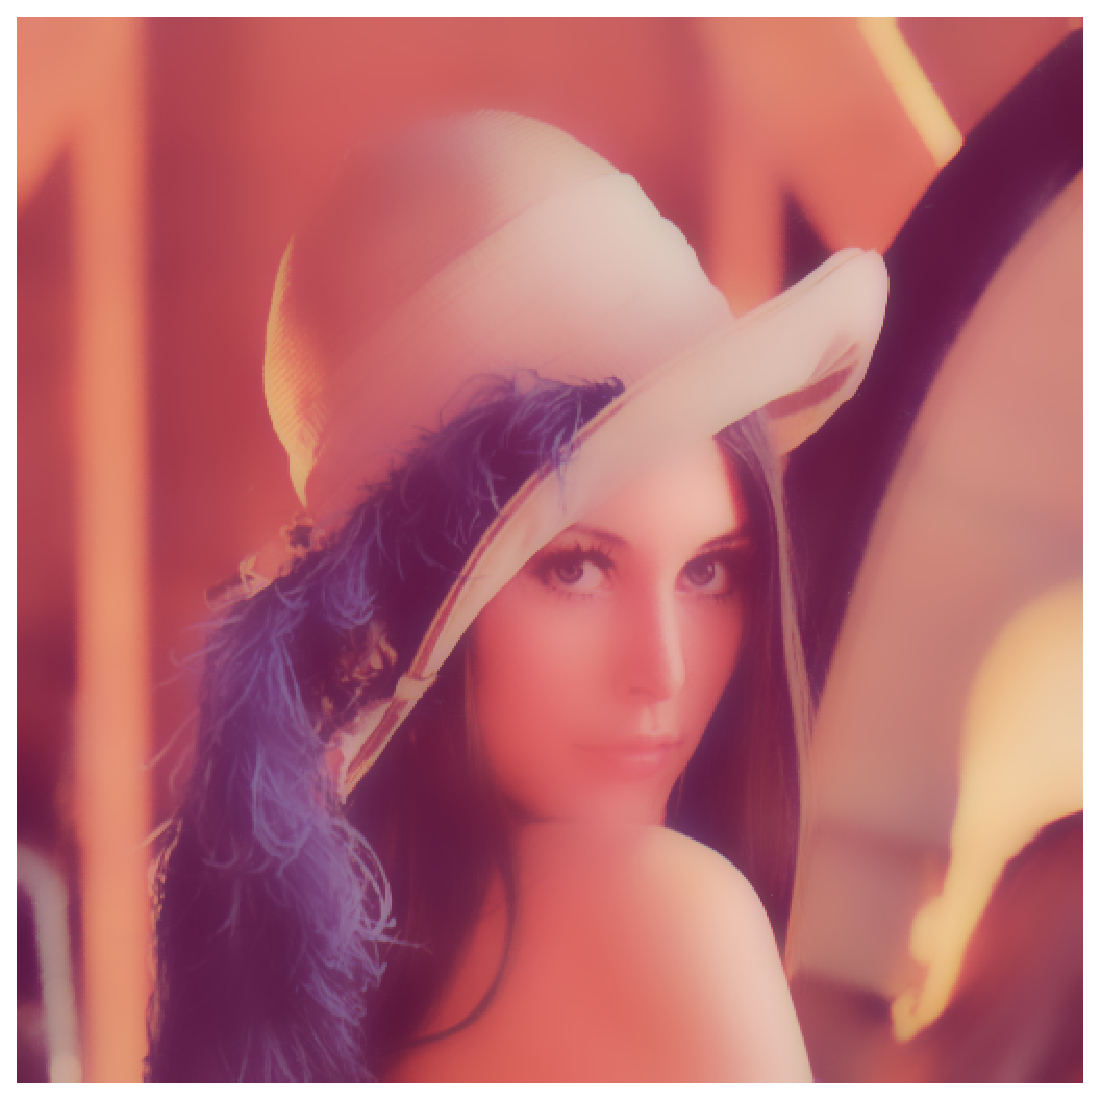
\includegraphics[scale=0.73]{Lenna_bf_100_10.eps} %TODO render with PDF
	%\end{center}
  %\caption{A subfigure}
  %\label{fig:sub2}
\end{subfigure}
\caption{An example of Gaussian blur with $\sigma$ = 10 (top right) and Fast O(1) Bilateral Filter (bottom) with $\sigma_s=100, \sigma_r=10$ applied to the Lenna test image (top left)\cite{lenna}.}
\label{fig_gaussian_blur}
\end{figure}
%\end{center}

\subsubsection{Naive bilateral filter algorithm}

The improvement introduced to the Gaussian filter by the bilateral filter is an additional weight term which takes into account the values of the $\sigma$-neighborhood of the pixel (see figures \ref{fig_gaussian_blur,fig_microscope} for an example). This requires the addition of another cycle over all the pixels in the image and leads us to the following formulation:

\begin{center}
\begin{algorithm}[H]
	\KwData{$I$ - input image, $O$ - output image, $\sigma$ - filter range, $h$ - height of the input image, $w$ - width of the input image}
	\For{$x = 1, 2, ... w$}{
		\For{$y = 1, 2, ... h$}{
			$O(x,y) = 0$

			$norm = 0$
			
			\For{$x_\sigma = x-\sigma ... x+\sigma$}{
				\For{$y_\sigma = y-\sigma ... y+\sigma$}{
					$norm += G_{\sigma_s}(\| (x_\sigma, y_\sigma)-(x, y) \|)G_{\sigma_r}(I(x_\sigma, y_\sigma)-I(x, y))$

					$O(x,y) += I(x_\sigma, y_\sigma)G_{\sigma_s}(\| (x_\sigma, y_\sigma)-(x, y) \|)G_{\sigma_r}(I(x_\sigma, y_\sigma)-I(x, y))$
				}
			}
			$O(x,y) = \frac{O(x,y)}{norm}$
		}
	}
\end{algorithm}
\end{center}

TODO correct the formulation

\subsubsection{Fast O(1) bilateral filter algorithm}

Since the bilateral filter it's previously defined form has a time complexity of $O(|I|^2)$ (with $|I|$ as the number of pixels in the image), it is easy to see that it is a feasible approach for only smaller images, as processing time grows quadratically as the image size increases. Therefore in order provide a relevant evaluation of distributed image processing with regard to large images, I selected an existing implementation of an optimised bilateral filter algorithm, described by Chaudhury et al. in "Fast O(1) bilateral filtering using trigonometric range kernels" \cite{chaudhury2011fast}. The authors also provide an existing Java implementationin the form of an ImageJ plug-in, which I adapted into a Hadoop MapReduce program in order to be able to directly compare sequential and distributed performance \cite{imagej}.

\subsection{Practical approach}

Due to the size of the image in question, the first step in the processing chain was to split it into parts small enough to fit into HDFS blocks, but big enough to maximally take advantage of the processing power: as each Map or Reduce task requires some resources to start and shut down, it is in our interests to minimise the number of these tasks. When running my experiments, I used a Hadoop cluster set up with a HDFS block size of 64 megabytes. Therefore, when splitting the big image into parts (each a PNG file), I used the following reasoning:

\begin{itemize}
\item A standard image of three color channels, 64 megabytes can hold values of $64*1024*1024*8/24\cong22369621$ pixels, which is roughly an image of 4729 by 4729 pixels.
\item Since this calculation is for estimating storage requirements for raw data, it can be safely assumed that even in the worst case scenario, PNG compression will not perform worse.
\item Therefore, a choice of 4500 by 4500 pixels should be close to optimal, regardless of the content of the image.
\end{itemize}

Before partitioning the image based on this idea, it is also necessary to take into account the characteristics of the processing we are about to apply. Namely, we have to ensure that the results of this divide-and-conquer type approach are identical to the results we would attain by processing the image without partitioning. In this case, we are dealing with a local non-iterative algorithm, therefore this is relatively straightforward: we only have to make sure that adjacent parts of the image have an overlap big enough, so that when the algorithm calculates new values for pixels at the edge of the partial images, it still has the values of their neighboring pixels. For example, in the case of applying Gaussian blur with a radius of 5, the initial image should be partitioned so that individual pieces have an overlap of at least 5 pixels.

\begin{figure}[h]
\begin{center}
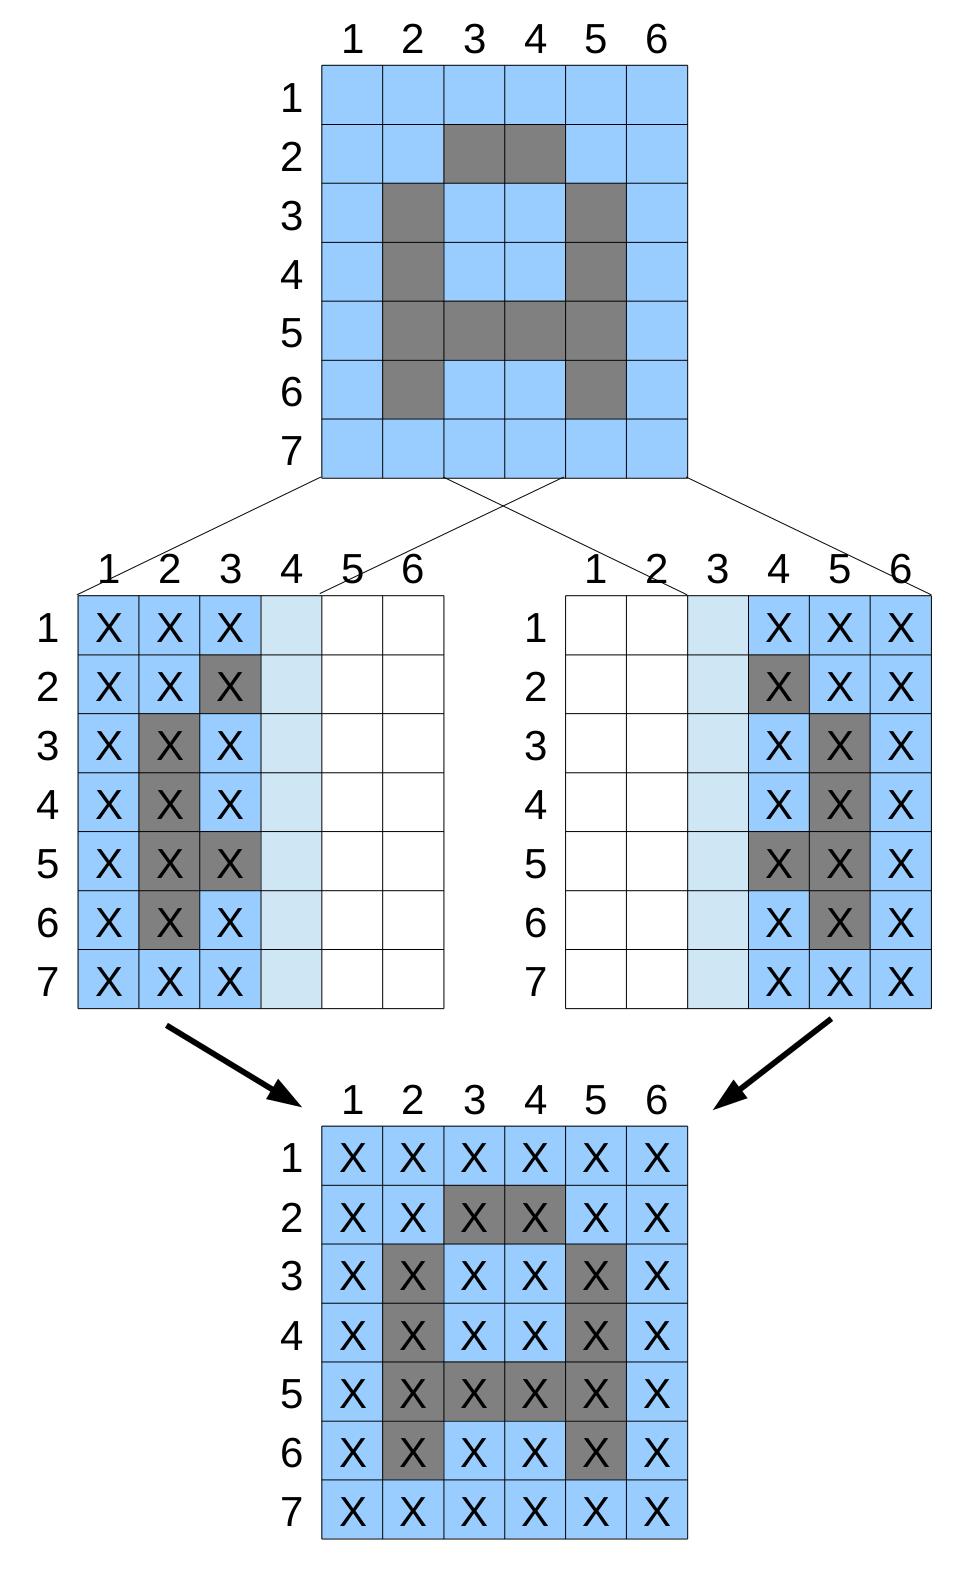
\includegraphics[scale=0.8]{partitioning.eps} %TODO render with PDF
%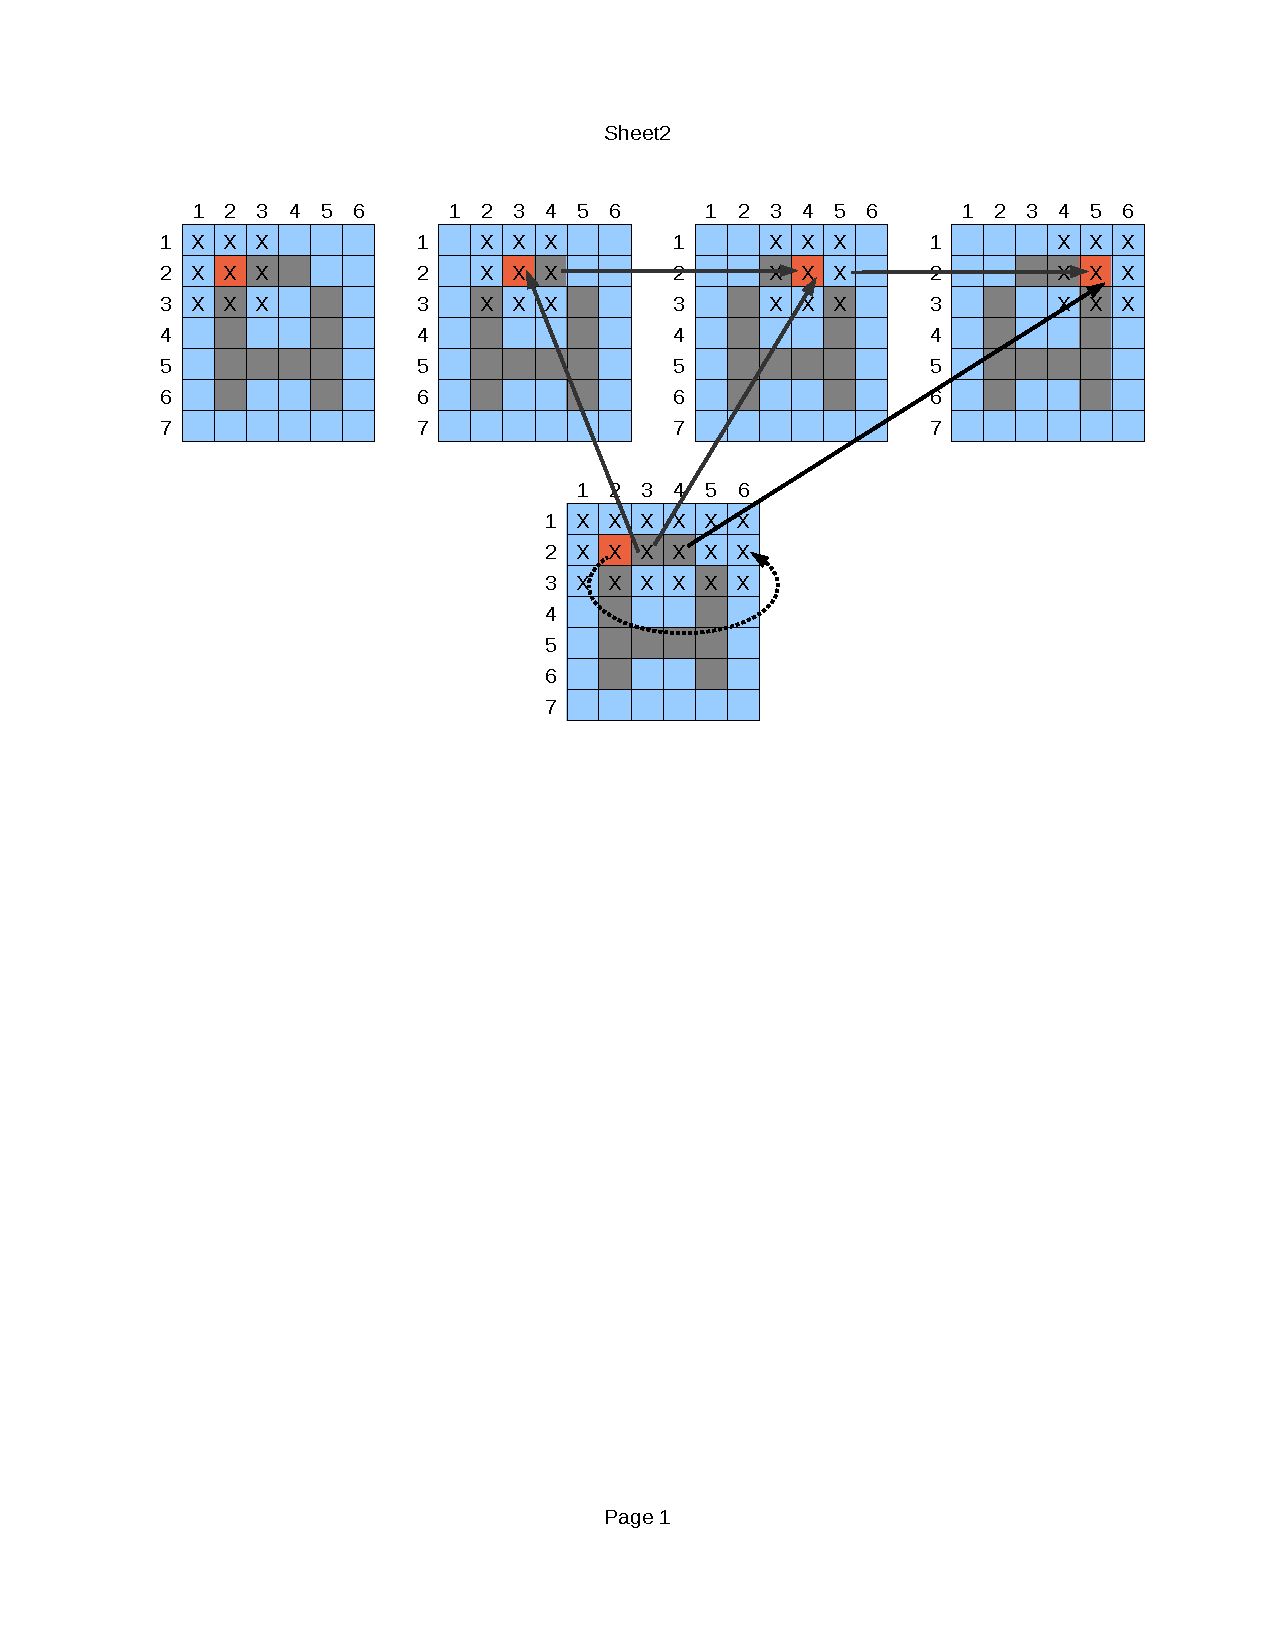
\includegraphics[scale=0.8]{local_iterative.pdf} %render with PDF
\caption{A diagram illustrating the concept of partitioning. Bright blue signifies the overlap necessary to calculate all the X-s on the left and right parts. Later the pieces can be merged and the overlap discarded.}
\label{fig_partitioning}
\end{center}
\end{figure}

In the spirit of this analysis, I split the 6.99 gigapixel photo into pieces using the following algorithm:

\begin{center}
\begin{algorithm}[H]
	\KwData{$w$ - input width, $h$ - input height, $o$ - overlap, $b$ - piece height/width, $f_x$ - width offset, $f_y$ - height offset}
	\For{$f_x = 0, 1, ... w$}{

		\If{$f_x + b > w$}{
			$tmp_{width} = w - f_x$			
		}
		\Else{$tmp_{width} = b$}

		\For{$f_y = 0, 1, ... h$}{

			\If{$f_y + b > h$}{
				$tmp_{height} = w - f_x$
			}
			\Else{$tmp_{height} = b$}
			
			$extract\_part(f_x, f_y, tmp_{width}, tmp_{height})$

			$f_y += b$
		}
		$f_x += b$
	}
\end{algorithm}
\end{center}

As a result, the original image was converted into 380 parts of varying size both in terms of dimensions and storage: the biggest piece with dimensions 4500 by 4500 and 30.4 megabytes in size, and the smallest piece being roughly 913 kilobytes with a width of 1381 and height of 601 pixels. This concludes the part of pre-processing the data in preparation of uploading it to the Hadoop Distributed File System.
To extract the pieces from the GeoTIFF container into individual PNG files, I used the Geospatial Data Abstraction Library (GDAL) in conjunction with a script written in Python specially for this purpose \cite{gdal}.

\subsubsection{Implementation with Hadoop}

Having partitioned the image into pieces that fit into memory, the next step is to design a MapReduce program to operate on this data. Since, by specifying overlaps and fitting the pieces within the HDFS block size during the partitioning phase, we have already ensured that each instance of the algorithm has it's necessary data locally available. Also, since we can easily perform all necessary computations in the Map phase, there is no need for a Reducer - Hadoop will simply write output to storage after the Map phase. Therefore, in this case, the MapReduce program consists only of three definitions: InputFormat, Mapper and OutputFormat. Their respective purposes are straightforward: read blocks from storage and convert them to Java objects that contain a piece of the image, process these pieces with the fast O(1) bilateral filter, and finally convert the resulting objects back to PNG files and write to HDFS. 

\subsubsection{Testing}

All tests were run on a Hadoop cluster with one m1.small virtual machine as the master node and m2.xlarge virtual machines as computing nodes on the Amazon EC2 cloud (see figure \ref{fig_instance_types} for details on the instance types). With regard to the configuration of the Hadoop cluster, most parameters remained set to the default values both in runs with version 0.20.2 and 1.0.3. The only exceptions were setting the HDFS block size to 64 megabytes, and setting the maximum memory for Map and Reduce tasks to 15 000 megabytes. The choice of m2.xlarge instances for computing nodes was directly influenced by the requirements of the algorithm - all attempts to run the tests with m1.small instances failed because there was not enough memory available. Using m2.xlarge eliminated these problems and due to the number of cores, also allowed simultaneous processing of two images. In the following, I will present the results of testing the fast O(1) bilateral filter algorithm in various configurations.

\begin{figure}[h]
\begin{center}
\begin{tabular}{r | l}
Instance type & m1.small \\
\hline
Memory & 1.7 GiB \\
CPU & 1 virtual core with 1 EC2 Compute Unit \\
Local storage & 160 GB \\
Platform & 64-bit \\
\hline\hline
Instance type & m2.xlarge \\
\hline
Memory & 17.1 GiB \\
CPU & 2 virtual cores with 3.25 EC2 Compute Units each \\
Local storage & 420 GB \\
Platform & 64-bit \\
\end{tabular}
\caption{Parameters of the m1.small and m2.xlarge instance types according to the Amazon EC2 official web page \cite{ec2_instancetypes}. One EC2 Compute Unit can be thought of as the equivalent of a 
1.0-1.2 GHz 2007 Opteron or 2007 Xeon processor.}
\label{fig_instance_types}
\end{center}
\end{figure}

The principal results of testing can be seen in figure \ref{bf_speedup}. In order to best compare the MapReduce adaptation of the algorithm to it's performance as a stand-alone ImageJ plugin, I wrote a shell script which started an ImageJ macro to sequentially process all the parts of the original image in a m2.xlarge instance. Since the technical parameters of the instance were identical to the computing nodes', this gives us a good estimate of how much the Hadoop framework affected the speed of the computations. As can be seen from the chart in figure \ref{bf_speedup}, the decrease in speed is noticeable, but small. Considering that Hadoop also provides fault-tolerance, load balancing and handles the distribution of data all by itself, it can be argued that this sort of approach to image processing has justified itself, and could reliably used as a solution for similar problems.

\begin{figure}[h]
\begin{subfigure}{.5\textwidth}
%\begin{center}
  \centering
  \includegraphics[scale=1.0]{bf_speedup.eps} %TODO render with PDF
  %\caption{Regular image}
  %\label{fig:sub1}
%\end{center}
\end{subfigure}
%
\\
\begin{subfigure}{.5\textwidth}
\begin{center}
  %\centering
	\begin{tabular}{c | c | c | c}
	Number of nodes & Wall time (s.) & Theoretical speed-up & Actual speed-up \\ 
	\hline
	Sequential & 22763.9 & 1 & 1 \\
	1 & 23879.5 & 1 & 0.95 \\
	2 & 11944.6 & 2 & 1.91 \\
	4 & 6534.2 & 4 & 3.48 \\
	8 & 3031.2 & 8 & 7.51 \\
	16 & 1557.2 & 16 & 14.62 \\
	\end{tabular}
\end{center}
\end{subfigure}
\caption{A comparison of processing time with regard to speed-up due to parallelisation. The left column represents the number of computing nodes in the cluster. The result is an average of ten runs with 8 and 16 nodes, five runs with 2 and 4 nodes and two runs with 1 node. Sequential represents the result attained by a stand-alone script calling ImageJ and running the Fast O(1) Bilateral Filter plugin on all pieces of the image.}
\label{bf_speedup}
\end{figure}

\begin{figure}[h]
\begin{center}
\begin{tabular}{c | c | c}
Number of nodes & Wall time, 0.20.2 (s.) & Wall time, 1.0.3 (s.) \\ 
\hline
8 & 3031.2 & 3286.9 \\
16 & 1557.2 & 1693.4 \\
\end{tabular}
\caption{Comparison in processing time between a cluster running on Hadoop version 0.20.2 and 1.0.3. In the latter case, the result is an average of five test runs.}
\label{fig_hadoop_version_compare}
\end{center}
\end{figure}

The results of comparing performance between Hadoop version 0.20.2 and 1.0.3 can be seen in figure \ref{fig_hadoop_version_compare}.

%\subsection{Technologies used}

%\subsubsection{ImageJ}
%For processing images while working on the practical part of this thesis, I used the ImageJ library. It is a freely available image processing application written in Java and developed by the National Institutes of Health \cite{imagej}. It supports the processing and analysis of a wide variety of image types (8-, 16-, 32-bit RGB/black \& white images) and many commonly used image file formats such as PNG, TIFF and JPEG.

\chapter{Summary}

In this thesis, I have described an approach to distributed image processing using the MapReduce model, along with two examples of practical application using the Apache Hadoop framework. I have also provided a general classification of image processing algorithms and explained some of the basic issues that should be taken into account when considering methods of parallelisation. When discussing all of these subjects, I have focused on two-dimensional images with three color channels, which is essentially the vast majority of data that is commonly thought of as an "image". Finally, I also make a distinction between the tasks of processing a large data-set of regular-sized images and one large image with regard to the previously defined classes of algorithms.
 
First, in the case of working with a data-set of regular images, there are almost no insurmountable issues with adapting any kind of algorithm to the MapReduce model. The divide-and-conquer approach of splitting up the data-set for independent processing works well in frameworks such as Hadoop, and - as shown in the practical example - there are almost no technical barriers for integrating MapReduce programs with software written in any language, as the list of supported platforms for Hadoop includes Linux, Windows, BSD, Mac OS/X and OpenSolaris \cite{hadoopfaq}. It is to be noted, though, that in my analysis, I did not consider any algorithms which require more than one image as input. This excludes, for example, clustering algorithms which need to compare images to each other. A potential theme for future work would be to determine in more detail the characteristics of these algorithms in order to see whether applying the MapReduce model is a good method of distributing this processing, or should altogether different solutions be proposed.

Moving on to the case of processing images, whose dimensions are large enough to require special attention regardless of the nature of the task itself, the applicability of MapReduce is less feasible. With local non-iterative algorithms, it suffices to split the input into pieces, process the pieces, and then assemble the final output image. The other three cases are not so trivial: the communication requirements of these algorithms imply running many MapReduce jobs, which is currently unfeasible when using Hadoop. However, these problems may be solved by using implementations of MapReduce that are more suitable for iterative processing, such as Twister, HaLoop or Spark, or increases in network bandwidth and latency \cite{ekanayake2010twister,bu2010haloop,zaharia2010spark}. 

\chapter{Future work}

\clearpage
\addcontentsline{toc}{chapter}{Bibliography}
\bibliographystyle{plain}
\bibliography{bibliography}

\end{document}
